% What is the domain // what is the current use // what are the current problems // what are the technical challenges // how did i meet these technical challenges // how did it work

\chapter{Visualization Application Design (contributions)} \label{cha:contributions}

This chapter describes the contributions of the papers that are included in this thesis.  This section describes the partition of papers into five different application domains and the subsequent sections contain each a description of the problem domain and then elaborate on the contributions of the included papers.

\textbf{Finite Element Models. } \paperFEM\ deals with algorithmic challenges to efficiently render non-linear finite element models, in this case exemplified on a high-resolution simulation of stress inside a heart muscle, a deformation model of the breast muscle, and a simultion of the muscle fibers in the tongue~(\SC{contributions:fem}).

\textbf{Deep Brain Stimulation. } \paperDBS\ describes an application system that is targeted to be used in deep brain stimulation interventions in order improve the placement of electrodes using a fusion of multiple data modalities in real-time~(\SC{contributions:dbs}).

\textbf{Urban Search \& Rescue. } \paperVMV, \paperSSRR, and \paperCGF\ portray the collaborative work on designing a visualization system to support urban search \& rescue operators and rescuers during the reconnaissance of partially collapsed buildlings.  The system utilizes acquired \nD{3} point cloud data as the basis for a path suggestion algorithm, whose results are presented to the expert user for a human-in-the-loop decision support of optimal building exploration in search for victims.~(\SC{contributions:usar})

\textbf{Space Weather. } The work presented in \paperCME\ describes a visualization application used to compare simulations and real world observations in the context of space weather.  Space Weather is the collective term for the study of the overall plasma conditions in our solar system and how they impact the Earth, humans, and satellites.~(\SC{contributions:spaceweather})

\textbf{Astrophysical Visualization. } \paperDSG, \paperGB, and \paperOS\  describe a visualization system called \emph{OpenSpace} that was designed with a focus on public dissemination of astronomical and astrophysical phenomen\ae.~(\SC{contributions:astro})

Each of the sections provide a short introduction into the domain and, then, elaborate on the work that has been done in the respective papers.





\section{Finite Element Models} \label{contributions:fem}
The work of \paperFEM\ describes the creation of an algorithm to efficiently render non-linear finite element models that traditionally require expensive calculations during the rendering to be represented correctly.  The paper describes an algorithm that utilizes an efficient storage and look-up of precalculated rays, thus improving the rendering performance by an order of magnitude.

\subsection{Domain and Scientific Problems} \label{contributions:fem:background}
Finite element models (FEM) methods are used extensively in a large number of fields, such as engineering, construction, or biology, as an approach to solve complex problems numerically by separating the problem domain into a finite number of cells, each with their own local coordinate system, over which the numerical simulation can be performed independently and efficiently.  Two coordinate systems are associated with each element; the location and deformation of an element is specified in Cartesian \emph{world coordinates}, whereas the computed values of the element are represented in a material coordinate system $\xi$ which, in most cases, is not Cartesian but can be of arbitrary geometry that simplifies the underlying computation (see Figures~\ref{contributions:fem:rays:world} and \ref{contributions:fem:rays:xi}).  The vertex coordinates of each element can be expressed in either coordinate system through a bilinear transformation; in many cases, however, an analytical solution does not exist for arbitrary coordinates inside the element and the transformation involves computationally expensive iterative solvers, such as the Newton method.  For more information on finite element models can be found in the book by Bathe and Wilson~\cite{bathe1976numerical}.

\begin{figure}
\centering
\begin{subfigure}[b]{0.3\textwidth}
    \centering
    \fbox{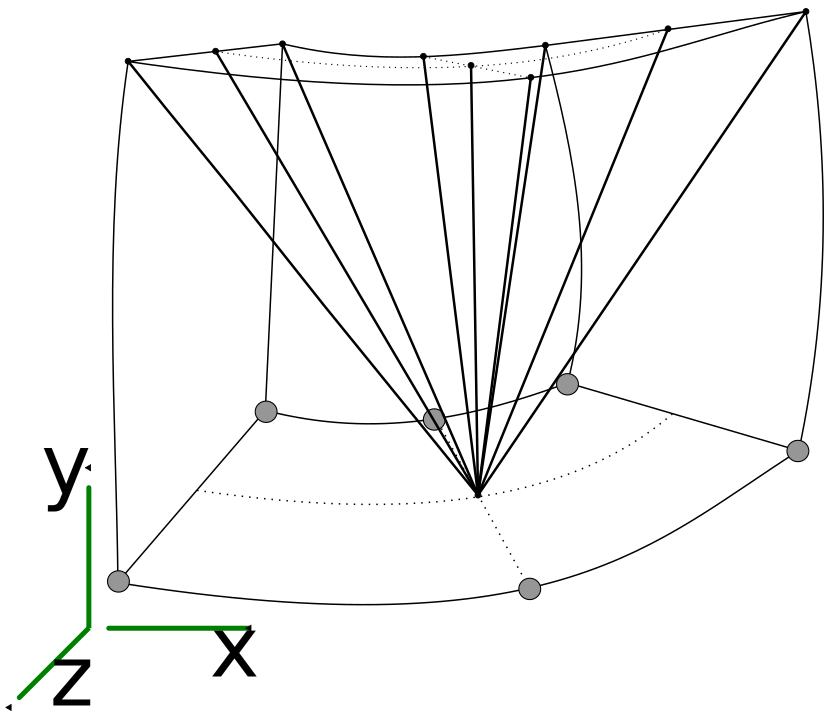
\includegraphics[width=\abfboximagewidth, height=4cm]{figures/contributions/fem/splines-world-space.pdf}}
    \caption{Rays and element geometry shown in Cartesian world space.}
    \label{contributions:fem:rays:world}
\end{subfigure}
\hspace*{0.15cm}
\begin{subfigure}[b]{0.3\textwidth}
    \centering
    \fbox{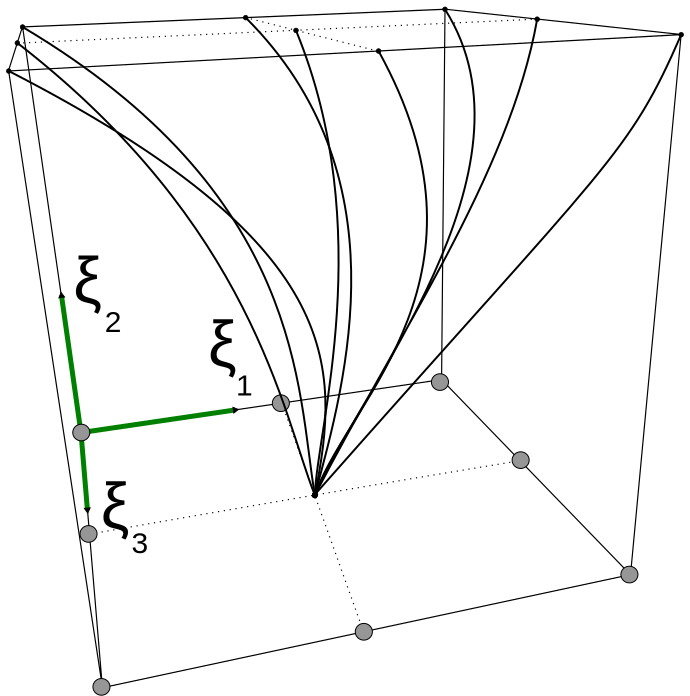
\includegraphics[width=\abfboximagewidth, height=4cm]{figures/contributions/fem/splines-xi-space.pdf}}
    \caption{Rays and element geometry shown in material space.}
    \label{contributions:fem:rays:xi}
\end{subfigure}
\hspace*{0.15cm}
\begin{subfigure}[b]{0.3\textwidth}
    \centering
    \fbox{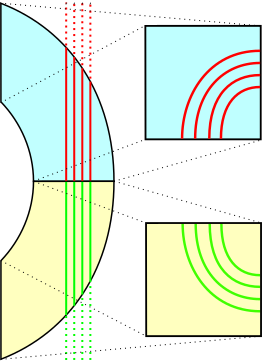
\includegraphics[width=2.91cm, height=4cm]{figures/contributions/fem/viewingrays.pdf}}
    \caption{Converting coordinate systems turns straight viewing rays into curved rays.}
    \label{contributions:fem:rays:rays}
\end{subfigure}
\caption{Transformation between world coordinates and material coordinates for a set of viewing rays when viewing the element geometry and the viewing rays from the world (a) or the material (b) coordinate system.}
\label{contributions:fem:rays}
\end{figure}

This work was mainly developed focussing of a simulation of a human heart that calculates the stress tensor at each location during the cardiac cycle.  By comparing the results of healthy and abnormal hearts, it becomes possible to detect structural defects before they manifest~\cite{young1992three, young1995tracking}. Traditionally, direct volume rendering techniques were not capable of visualizing these datasets and instead iso-surfaces or glyphs have been used~\cite{wunsche2003visualization}.

When performing direct volume rendering on the FEM dataset, view rays for each pixel are defined in world coordinates and are straight lines in world coordinates.  For each element that is intersected by a ray, all rays have to be converted into the material space in order to be able to sample the values, which are given in $\xi$ material space.  \fref{contributions:fem:rays:rays} shows an example of the ray transformations from a Cartesian world space into a bicubic-linear material space.  Converting each sample point from Cartesian space into material space using an iterative solver is prohibitively expensive for real-time use.


\subsection{Application Requirements} \label{contributions:fem:requirements}
For each viewing ray, a large number of sampling points have to be retrieved for a correct front-to-back composited image that reduces sampling artifacts.  The additional coordinate transform during the data access becomes a bottleneck in the case of non-linear FEM datasets that reduces rendering speeds to non-interactive frame rates.  \paperFEM\ describes an algorithm that utilizes a precomputation step to cache a reduced set of possible rays that are then used in the rendering step to efficiently access the data, resulting in a $15\times$ performance gain, relative to straight-forward GPU implementations, which in turn, are an improvement of 2 to 4 orders of magnitude compared to a CPU implementation~\cite{liu12gpu}.


\subsection{Algorithm} \label{contributions:fem:algorithm}
\begin{figure}
\centering
\includegraphics[width=\textwidth]{figures/contributions/fem/workflow.pdf}
\caption{The workflow employed in the finite element model volume rendering algorithm.  The first two steps are precomputing potential ray paths through the volume that increase the performance during the third step.}
\label{contributions:fem:workflow}
\end{figure}

In order to improve the performance of the rendering, the expensive coordinate transformations have to be computed offline prior to the rendering and then retrieved efficiently.  The algorithm described in \paperFEM\ utilizes a Catmull-Rom spline-based ray representation , which can be efficiently stored and retrieved at rendering time~\cite{catmull1974class}.  A number of approximation steps are performed in order to increase the similarity between different rays and represent these by a reduced set of \emph{proxy rays}, which drastically reduces the number of rays that need to be stored and still maintain a high quality rendering.  \fref{contributions:fem:workflow} shows the algorithm's workflow in detail, with the first two steps being precomputed once for each finite element model in order to improve the performance of the third real-time rendering step.  The algorithm's 5 steps are described in the following sections:
\begin{description}[leftmargin=10em,style=nextline]
  \item[Point Generation]  A fixed number of points are generated for all faces of each element.  For each point, a \emph{proxy ray} is created to every other point in the same element but not the same face.
  \item[Ray computation]  The \emph{proxy rays} for each pair of points is sampled using a fixed sampling rate that is independent from the rendering sampling rate.  For each sample, the expensive coordinate transformation is performed).
  \item[Curve Similarity]  Through renormalization and alignment, the similarity between all \emph{proxy rays} is improved without losing information.
  \item[Curve Clustering]  Using k-means clustering, a representative subset of \emph{proxy rays} is created.  Each original entry-exit point pair references its new representative path.
  \item[Rendering ]  For each viewing ray, the \emph{proxy rays} are used to sample the correct locations in material space without the need for the expensive coordinate transformation.
\end{description}

The following two sections describe the curve clustering and the rendering;  the point generation and the ray computation steps are described in \paperFEM.

% \subsubsection{Proxy Ray Generation} \label{contributions:fem:proxyray}
% First, we do not store the entirety of a proxy ray, but sample it in a few points and use these as control points for a Catmull-Rom spline from which we can reconstruct the original path. The number of control points that are used to approximate each ray is a user-defined parameters. The optimal parameter for this value depends on the complexity of the dataset (see \SC{contributions:fem:results}). 

% Second, we compute only a finite number of proxy rays for each element by creating a uniform grid on each of the elements surface and computing all proxy rays between pairwise combinations of grid points. Figures~\ref{contributions:fem:rays:world} and~\ref{contributions:fem:rays:xi} show a potential set of these rays for an element in world coordinates and material space. We can apply this approximation since well-behaved finite element simulations usually do not produce degenerate elements for which a much higher resolution is needed.


\subsubsection{Curve Clustering} \label{contributions:fem:curves}
\begin{figure}
\centering
\fbox{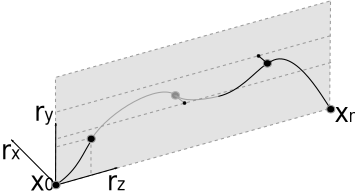
\includegraphics[width=0.75\textwidth]{figures/contributions/fem/splinetransformation.pdf}}
\caption{Increasing the similarity between splines through a lossless conversion into a common coordinate system.}
\label{contributions:fem:splines}
\end{figure}

A sampling of the $|F|$ faces of the $|E|$ elements of the model using $n$ points per face results in $r_t = \left( n^2 \cdot |F| \right) ^2 \cdot |E|$ proxy rays.  Without further reductions this number is prohibitely large to store all precomputed rays on the GPU.  However, since there is a potential for a high degree of similarity between rays due to symmetries in the finite model elements and bounded ray complexity as each ray has to stay inside the boundaries of an element.  Thus, it is possible to utilize a clustering algorithm to reduce the number of representative \emph{proxy rays} necessary during the rendering without introducing large errors.

% \begin{figure}
% \centering
% \begin{subfigure}[b]{0.4\textwidth}
%     \fbox{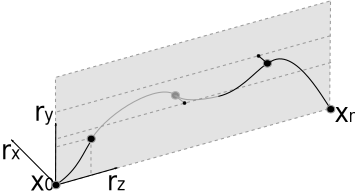
\includegraphics[width=0.99\textwidth]{figures/contributions/fem/splinetransformation.pdf}}
%     \caption{Increasing the similarity between splines by converting them into a common coordinate system.}
%     \label{contributions:fem:splines}
% \end{subfigure}
% \hspace{2cm}
% \begin{subfigure}[b]{0.4\textwidth}
%     \fbox{\includegraphics[width=0.99\textwidth]{figures/contributions/fem/metric.pdf}}
%     \caption{A representation of the metric that is used in the K-Means clustering algorithm, approximating the area between the two rays by a sum of the triangleresponders to manually create a map  areas.}
%     \label{contributions:fem:metric}
% \end{subfigure}
% \end{figure}

The first step is to increase the similarity between proxy rays while maintaining the ability to uniquely reconstruct the final ray.  For this, all rays are rotated and stretched such that the first point $P_1$ is equal to $(0,0,0)$ and the last $P_n$ control point is equal to $(0,0,1)$.  Then, all control points are rotated by a rotation angle $\theta$ around the $z$ axis such that the first point $P_i$ that is not collinear with $P_1$ and $P_n$ is in the $yz$ plane.  \fref{contributions:fem:splines} shows the results of these transformations on an example ray.  The translation and the scaling are undone during the rendering step without storing additional information, as the entry and exit points (and their distance) are known.  Only the angle $\theta$ needs to be recorded for each \emph{proxy ray}.

\begin{figure}
\centering
\includegraphics[width=0.75\textwidth]{figures/contributions/fem/metric.pdf}
\caption{A representation of the metric that is used in the k-means clustering algorithm, approximating the area between the two rays by a sum of the triangle areas.}
\label{contributions:fem:metric}
\end{figure}

For the clustering of the splines, we make use of the variant of the k-means~\cite{hartigan75kmeans} algorithm because of its stability and ability to deal with values of an arbitrary number of dimensions.  We adapt an idea from Abraham~\etal \cite{abraham03clustering} and perform the clustering directly on the control points of the Catmull-Rom splines.  The distance metric for the clustering uses the area between two curves as approximated by a Riemann sum of triangles connecting the proxy rays, sampled at a high frequency (see~\fref{contributions:fem:metric}).  For two proxy rays $a$ and $b$, and their $n$ sampled points $\vec{a_1}, \dots \vec{a_n}$ and $\vec{b_0}, \dots \vec{b_n}$ with $\vec{a_1} = \vec{b_1}$, $\vec{a_n} = \vec{b_n}$, $\exists i\in[2, n-1] : \vec{a_i}_x = 0$, and $\exists j\in[2, n-1] : \vec{b_j}_x = 0$ due to the transformation performed in the last paragraph, the similarity metric is defined as:

\begin{eqnarray}
d(a,b) &=& \frac{1}{2} \Big( \Vert \overline{\vec{a_1}\vec{a_2}} \times \overline{\vec{a_2}\vec{b_2}}\Vert + \nonumber \\
&& \sum_{i=2}^{n-2}\Vert \overline{\vec{a_i}\vec{a_{i+1}}} \times \overline{\vec{a_i}\vec{b_i}} \Vert + \Vert \overline{\vec{b_i}\vec{b_{i+1}}} \times \overline{\vec{b_{i+1}}\vec{a_{i+1}}}\Vert + \\
&& \Vert \overline{\vec{a_{n-1}}\vec{a_n}} \times \overline{\vec{a_{n-1}}\vec{b_{n-1}}}\Vert \Big) \nonumber 
\end{eqnarray}

Using this metric, all proxy rays are then clustered into $k$ representatives.  For each proxy ray, an identifier for the representative, as well as the angle $\theta$ is stored.



\subsubsection{Rendering} \label{contributions:fem:rendering}
\begin{wrapfigure}{o}{0.4\textwidth}
\centering
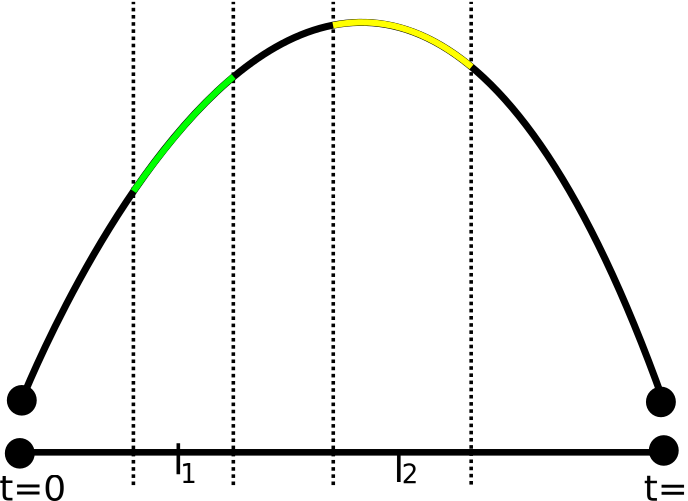
\includegraphics[width=0.39\textwidth]{figures/contributions/fem/arclength.pdf}
\caption{The desire to uniformly sample the view ray in world space requires an arclength parametrization of the proxy ray.}
\label{contributions:fem:arclength}
\end{wrapfigure}

During the rendering step of the algorithm, the geometries for all elements of the finite element model are rendered.  Its coordinates are mapped to the RGB channel, as described in the DVR technique by Kr\"uger and Westermann~\cite{kruger2003acceleration}, and the face identifier and element identifier are encoded in the transparency channel.  The entire scene is then rendered in multiple passes, employing a modified depth peeling approach as described by Everitt~\cite{everitt2001interactive} for each rendering pass.  In each pass, the entry and exit point geometries are rendered which trigger the fragment shader of the GPU that performs the rendering as described in the rest of this section.

\begin{figure}
    \centering
    \includegraphics[width=0.5\textwidth]{figures/contributions/fem/heartfine.jpg}
    \caption{The insets show potential rendering artifacts when applying the depth peeling algorithm to finite element methods.}
    \label{contributions:fem:peeling}
\end{figure}

For each of the peeling steps, the color information for every pair of fragments is used to access entry and exit points, the face, and element ID.  Using this information, the cluster ID and the angle $\theta$ of the proxy ray that is closest to the fragment pair is retrieved.  The previous transformations of the proxy ray are undone by scaling the proxy ray by the distance between the entry and exit points in world coordinates, translating and rotating the ray such that $P_1$ coincides with the entry point and $P_n$ coincides with the entry point, and then rotating the proxy ray around the axis connecting $P_0$ and $P_n$ by $\theta$.

\begin{wrapfigure}{o}{0.4\textwidth}
\centering
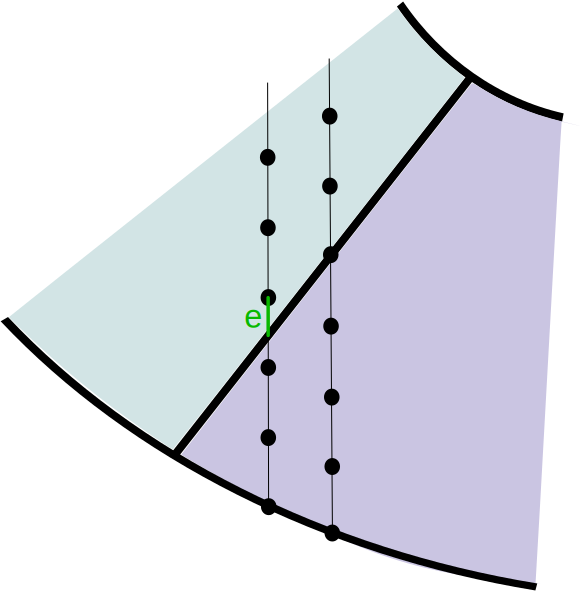
\includegraphics[width=0.39\textwidth]{figures/contributions/fem/overshoot.pdf}
\caption{Special border handling is required between elements, as a na\"{i}ve implementation would oversample the boundary.}
\label{contributions:fem:overshoot}
\end{wrapfigure}

The ray marching then interpolates along the Catmull-Rom spline to retrieve the correct sampling value in material space.  The stepsize $h$, however must not be constant in the material space $\xi$ as this would lead to a non-uniform sampling in world space (see~\fref{contributions:fem:arclength}). Therefore, the spline interpolation parameter $t \in [0,1]$ has to be converted into an arclength parametrization such that the sampling in material space becomes non-uniform to make the world space sampling uniform instead~\cite{guenter90arclength}.  A second subtle error occurs at the boundary between elements and is exemplified in \fref{contributions:fem:overshoot}.  Starting the ray marching at the beginning of each element would also lead to a non-uniform sampling across element boundaries and thus introduce rendering artifacts.  For this reason, the remaining distance between the last sample and the exit point is stored at the end of the ray marching and this distance is used to offset the first sampling point in the following element, similar to the method employed by Ljung \etal~\cite{ljung2006adaptive}.

\begin{figure}
\centering
\begin{subfigure}[b]{0.4\textwidth}
    \includegraphics[width=\abfboximagewidth]{figures/contributions/fem/heart-5.jpg}
    \caption{Using no inter-ray or intra-ray interpolation.}
    \label{contributions:fem:raw}
\end{subfigure}
\hspace{2cm}
\begin{subfigure}[b]{0.4\textwidth}
    \includegraphics[width=\abfboximagewidth]{figures/contributions/fem/heart-5-rr-ii.jpg}
    \caption{Using inter-ray and intra-ray interpolation.}
    \label{contributions:fem:interpolation}
\end{subfigure}
\caption{A volume rendering of the heart dataset using $5\times 5$ rays per face for each element showing the difference between the interpolation schemes.}
\label{contributions:fem:interpolationexample}
\end{figure}

A low sampling resolution of proxy rays introduces rendering artifacts as the same proxy rays will be used for a large area of the face; similar to nearest neighbor interpolation.  In order to mitigate these artifacts, we introduce a bilinear interpolation of control points of the four closest proxy rays and perform the ray marching along the spline generated by these interpolated control points.  This interpolation method is called \emph{inter-ray interpolation}.

A second mitigation of low sampling rate utilizes the fact that the precomputation step considers ray between entry point $e$ and $f$ $r_{ef}$ independently from the ray $r_{fe}$.  This makes it possible to sample $r_{ef}$ with the sampling parameter $t$ and $r_{fe}$ using $t' = 1 - t$ and averaging the results before sampling the volume.  This method is called \emph{intra-ray interpolation}.  \fref{contributions:fem:interpolationexample} shows the difference using the two interpolation methods, where $5\times 5$ rays per face for each element were generated.






\section{Deep Brain Stimulation Interventions} \label{contributions:dbs}
\paperDBS\ describes the work in developing a medical visualization application for deep brain stimulation~(DBS)~intervention support in collaboration with physicians at the St.~Barbara Hospital in Hamm, Germany.  This system was designed to support the brain surgeon during an electrode placement surgery in order to achieve a higher precision and thus a higher probability of a positive outcome for the patient.



\subsection{Domain and Scientific Problems} \label{contributions:dbs:background}
Deep Brain Stimulation (DBS) is a form of medical intervention that targets, among others, patients afflicted with Parkinson's Disease or other forms of essential tremors.  During these interventions, an electrode is inserted into patient's brain that stimulates the surrounding regions by using an electric field.  Depending on the exact location and geometry of the electrode, different regions of the brain are stimulated, which has the potential to inhibit some of the debilitating effects of these tremors~\cite{lindberg2002impact}.  One target region for the treatment of tremors are the patient's subthalamic nuclei~(STN), which are two structures with the size of a few millimeters located deep in each hemisphere of the brain~\cite{benabid2009deep, richter2004determining}.  Using traditional imaging techniques such as CT or MRI, the exact location of an individual patient's STN can be difficult to determine~\cite{starr2002implantation}.  This procedure is further complicated as a small deviation in the electrodes' locations will excite other parts of the brain that can lead to side effects, such as memory loss or speech impairment.

Microelectrode Recordings (MER) have been developed to augment imaging modalities and make use of a cluster of recording electrodes that are capable of detecting the electric activities in the brain~\cite{lenz1988methods}.  The amplitude and frequency of the electric fields measured by the electrodes correlate with specific brain regions and can thus be used to determine whether the electrodes are in the correct location~\cite{benazzouz2002intraoperative}.  Currently, the results of the MER are reviewed by the surgeon on loudspeakers in the operating room.  Aside from the obvious drawbacks of a limited auditory channel, a limited echoic memory, and potential background noise, a big challenge is the surgeon's mental separation between the spatial location of the electrodes and the results of their measurements, requiring the surgeon to keep a mental model of the brain regions and comparing those to a standard atlas in their head.  The same argument applies to the absolute location of the electrode cluster as well as the relative position of the electrodes inside the cluster.

A DBS intervention is performed in three distinct phases.  In the first phase, the \emph{planning} phase, the surgeon plans the operation at his workstation by locating and segmenting the most probable location of the STN using preoperative CT and MRI scans.  This information is used to plan an optimal access channel which evades important sensitive brain regions and selects the optimal location for the electrode to affect the~STN~\cite{butson2007patient}.  In the second phase, the \emph{recording} phase, the patient is in the operating room with a stereotaxic frame that provides mounts for the instruments is fixed to their head and which is visible on all scanning modalities and thus allow for a fixed-body transformation between the patient's head and the operating room.  The MER electrode cluster is inserted into the patient's brain along the preplanned access path until they have reached the predicted STN location.  During this phase, the measurements of the electrodes are used to discriminate the different brain regions and verify that the STN has been reached.  If the electrodes correctly identify the location of the STN, the electrodes' position along the access path is noted and their position relative to the stereotaxic frame is verified using bi-planar X-ray scans.  After this verification, the electrodes are retracted.  In the third phase, the \emph{placement} phase, the transmitting electrode is inserted into the same location that was determined in the previous phase, which is also verified using bi-planar X-ray scans.  The exact placement and the output of the electrode is modified using tests that examine the patient's ability, such as long term memory recall or measuring the amount of tremor.  This part of the procedure is challenging as the patient is awake during the entire procedure, which can last up to 10 hours.



\subsection{Application Requirements} \label{contributions:dbs:requirements}
Previous methods do not provide the surgeon with a system that sufficiently fuses the available information during the procedure.  Preoperative CT and MRI scans, interoperative X-ray scans, the electrode measurements during the insertion, and the final patient tests are all inspected independently and the surgeon has to maintain a mental correlation between all data sources, leading to fatigue, delays, and potential errors.  The collaboration partners desired a system that can ingest the access path planned using other sophisticated tools (see~\fref{contributions:dbs:planning}), the various scans (T$_1$ and T$_2$ MRI, CT, and X-ray), the MER measurements, as well as the patient tests during the operation and display them in a linked application.  Furthermore, a more effective visual encoding of the MER and the patient tests was desired by the surgeons.

There were a number of technical challenges that had to be addressed while designing the system;  1. An automated classification of the MER signals has to be displayed to the surgeon in context of the preoperative and interoperative CT, MRI, and X-ray scans.  2. A visual representation that enables the surgeon to interpret individual MER signals from the electrodes must be made available.  3. The system must contain a visual representation of the information gathered during the placement phase of the intervention, making it possible for the surgeon to visually correlate the information from the patient tests and X-ray scans.

Addressing these challenges requires the design of a system combining multiple linked views.  The following sections describe these views in greater detail.


\subsection{Contextual View} \label{contributions:dbs:contextual}
\begin{figure}
  \centering
  \fbox{\includegraphics[width=0.65\textwidth]{figures/contributions/dbs/contextual.png}}
  \caption{The contextual view provides the user with information about the location of the electrode relative to the patient's brain as well as the detected brain regions.}
  \label{contributions:dbs:contextual}
\end{figure}

This \nD{3} view combines preoperational CT and MRI scans with the bi-planar X-rays and the current electrode location (see~\fref{contributions:dbs:contextual}).  The view contains a multimodal volume rendering that shows the head and brain using T$_1$ and T$_2$-weighted MRI scans, the patient's skull extracted from the CT scan, and the interoperational X-ray scans as orthogonal planes.  The user chooses a vertical clipping threshold for T$_1$ scan and a separate threshold for the T$_1$ and the CT scan, making it possible to inspect only the T$_2$ scan of the brain while maintaining the context provided by the T$_1$ and CT scans.  The clipping is performed using the skull stripping algorithm described by Beyer~\etal~\cite{beyer2007high}.  The outermost layer contains a yellow band that shows the projected depth of the intended target location.  The planned access path is removed from the datasets and a single representative electrode is rendered at the correct location along this path.  The electrode provides the necessary spatial relation to the string of beads that are inserted into the path for each successful detection of a brain area by the MER.  Additionally, it prevents a dangerous left-right mismatch error that might otherwise occur during the operation in which the electrode is accidentally inserted into the wrong hemisphere.  This metaphor has already been used in similar systems when applied to non-human primates~\etal~\cite{miocinovic2007stereotactic} and presents the user with a visual representation of the various brain region the electrode has passed.  In order to improve the user's depth perception, the view uses a depth darkening effect that was presented by Luft~\etal~\cite{luft2006image}.  In addition to the electrode position as recorded by the instruments, this view also shows a reconstructed position of the electrode using the bi-planar X-ray scans which can be used by the surgeon to verify the correct placement position.  Lastly, this view also contains a separate horizontal indicator that presents the location of the electrode as well as the detected brain regions to the user without occlusion.



\subsection{Audio visualization} \label{contributions:dbs:audio}
\begin{figure}
\centering
    \begin{subfigure}[b]{0.49\textwidth}
        \fbox{\includegraphics[width=\abfboximagewidth]{figures/contributions/dbs/audio-signal.png}}
        \caption{The \nD{2} oscilloscope rendering of the direct electrode measurements.  Measurements with low amplitude are deemphasized by using darker colors.}
        \label{contributions:dbs:sound:2d}
    \end{subfigure}
    \hfill
    \begin{subfigure}[b]{0.49\textwidth}
        \fbox{\includegraphics[width=\abfboximagewidth]{figures/contributions/dbs/recording-3dsound.png}}
        \caption{The spatial \nD{3} rendering of the electrode rendering, showing their relative spatial location and rendering the high-amplitude measurements of the signal as colored discs.}
        \label{contributions:dbs:sound:3d}
    \end{subfigure}
    \caption{The two rendering methods for displaying the measurements recorded by the MER electrodes.  The views show the accurate values as well the relative spatial relation between the electrodes with an abstrct representation of the measurements.}
    \label{contributions:dbs:sound}
\end{figure}

The visual representation of the MER measurements is displayed to the user in two separate views.  The collaborators of the project used a microelectrode cluster that contains five electrodes, each of which is recording a separate signal from their specific location.  Thus, correlating the difference in measurements between electrodes provides information about the borders between brain regions, making it important to register the measurement locations.  A combination of two views presents the user with the MER measurements and at the same time provides the spatial mapping between recording and electrode location.

The first view shows an augmented visualization similar to an oscilloscope that presents the direct measurements from the electrodes.  As only the amplitude and frequency are relevant to the user during the procedure, we emphasize measurements that exceed a user-defined threshold and deemphasize the values below that threshold~(see~\fref{contributions:dbs:sound:2d}). This highlights potentially important measurements and reduces the noise from the low intensity signals.

The second view displays a \nD{3} representation of the electrodes' orientations and their measurements~(see~\fref{contributions:dbs:sound:3d}).  The camera orientations of this view and the \emph{Contextual View} are linked such that the mental registration between the two views is not broken.  In this view, each electrodes' measurements that exceed a user-defined threshold are shown as concentric discs that start at the electrodes moving away from the base with increasing time.  The size of the disc corresponds to the amplitude of the detected signal and thus show the strength of the measured signal.  This enables the surgeon to inspect the amplitude and frequency for each electrode in their current spatial location.  The color of each disc is determined by the classification algorithm that is used on the beads in the \emph{Contextual View}, but is simplified to only distinguish whether the electrode is inside or outside the STN.




\subsection{Target closeup} \label{contributions:dbs:target}
\begin{figure}
\fbox{\includegraphics[width=\abfboximagewidth]{figures/contributions/dbs/screenshot-target.jpg}}
\caption{The views that show the results of the different measurements performed during the recording phase. The \emph{Target closeup} (bottom view) contains the segmented location of the STN is visible as well as the results of the different tests at their spatial location.  The \emph{Placement guide} shows the likelihood measurements according to their depth along the access path.}
\label{contributions:dbs:target}
\end{figure}

After determining the potential electrode location, the closeup view, which is centered around the segmented location of the STN, combines all information that is relevant to the surgeon for the final placement of the stimulating electrode~(see \fref{contributions:dbs:target}).  Embedded in this view are the locations of the electrode as determined by the instrument's depth along the access path and the reconstructured location using the biplanar X-ray scans.  On demand, the surgeon can further enable the rendering of the MRI T$_2$-weighted MRI scan of the area.  In addition, it shows the recorded MER signal results as a red-green overlay on the backside of the bounding box and presents options to add the results of patient tests as additional transparent oval overlays.  All values show an estimate of their unknown uncertainty in this view that provide the surgeon with the information for a potential final placement that agrees with most measurements.


\subsection{System} \label{contributions:dbs:system}
\begin{figure}
  \centering
  \fbox{\includegraphics[width=0.85\textwidth]{figures/contributions/dbs/planning.png}}
  \caption{This view shows the part of the system that is used to import the results of a different planning tool to determine the entry point for the access path and the intented target location.}
  \label{contributions:dbs:planning}
\end{figure}



% \begin{figure}
% \centering
% \begin{subfigure}[b]{0.49\textwidth}
%     \fbox{\includegraphics[width=\textwidth]{figures/contributions/dbs/recording-3d-1.png}}
% \end{subfigure}
% \hfill
% \begin{subfigure}[b]{0.49\textwidth}
%     \fbox{\includegraphics[width=\textwidth]{figures/contributions/dbs/recording-3d-2.png}}
% \end{subfigure}
% % \includegraphics[width=\textwidth]{figures/contributions/dbs/recording-3d.png}
% \caption{Presenting the \emph{Contextual View} that shows the multimodal fusion of all available datasets. The preoperative CT and MRI as well as the interoperative bi-planar X-ray scans are visible together with the animated location of the electrode. The colored beads along the access path show an automatic classification of the electrode measurements.}
% \label{contributions:dbs:contextual}
% \end{figure}


The application resulting from this collaboration combines an enhanced multimodal \nD{3} volumetric rendering environment with the spatial visualization of electric measurements that are recording the patient's brain activity during the procedure in combination with patient-specific ability tests.  Spatially embedding the measurements with the volumetric information reduces the cognitive load of the surgeon during the surgeon, as this mental link does not have to be performed by the surgeon themself.  Furthermore, the system shows the uncertainties of different modalities in a single view, thus enabling the surgeon a comprehensive view and more insight during the procedure.


\subsection{Evaluation} \label{contributions:dbs:evaluation}
We performed an initial evaluation of the system using a qualitative user study with five neurosurgeons, which all had experience with conducing DBS interventions.  Each of the participants watched the usage of the system during the planning, recording, and placement phase.  The data for this test case was recording during an operation performed by one of the coauthors.  Then, each participant answered a questionnaire that used eight of the questions suggested by Martelli~\etal for evaluating computer-aided surgery systems~\cite{martelli2003criteria} with an additional free form text field for comments.  For each question, the participants could choose their reply on a 3-point Liekert scale~\cite{likert1932technique}.  The feedback from the experts was overall positive, with even the least positive participant agreeing to the majority of provided statements.  More information about the evaluation can be found in \paperDBS.






\section{Urban Search \& Rescue} \label{contributions:usar}
The work presented in \paperVMV, \paperSSRR, and \paperCGF\ was developed in the domain of \emph{Urban Search \& Rescue}~(USAR), a field of civil security that involves the location and extraction of victims that are trapped in collapsed buildings.  The goal of the work was to design a visualization application in collaboration with the Myndigheten f\"or samh\"allsskydd och beredskap, the Swedish Civil Contingencies Agency, that expedites the location and extraction of vicims in buildings through the use of sensor-equipped autonomous drones.

\subsection{Domain and Scientific Problems} \label{contributions:usar:background}
Traditionally, in the case of a partial building collapse in an urban environment, a country's civil contingency agency will perform an USAR operation in order to search the building for potentially injured survivors or victims and perform a rescue of these victims.  This operation entails \emph{responders} to enter the building being directed and coordinated by an \emph{incident commander}~(IC).  The major obstacle during these rescue operations is the fact that previous structural plans of the building are no longer usable and new unknown hazardous environments may have been created by the incident.  In addition, the viewing distance is usually restricted as debris and smoke impede the responders' progress.  During the rescue operation, the IC relies on the descriptions of the responders to manually create a map~(see \fref{contributions:usar:map:hand}).  This map is important for the IC in order to;  1. optimally coordinate the rescuers as time-to-rescue is the dominating factor in determining victims' survivability;  2. due to the collapse entire parts of the building might be inaccessible without removing rubble.  These \emph{voids} are prime locations of trapped victims and their detection on an unstructured \nD{2} map is difficult.

\begin{wrapfigure}{o}{0.4\textwidth}
\centering
\fbox{\includegraphics[width=0.38\textwidth]{figures/contributions/usar/map_drawing.jpg}}
\caption{A drawn map is the state-of-the-art method for coordinating multiple rescuers.}
\label{contributions:usar:map:hand}
\end{wrapfigure}

The robotics community, for a long time, has been advancing research into drones equipped with sensors and autonomous control in the usage for urban search \& rescue~\cite{liu2013robotic} that enable the improvement of the current workflow and creation of a system that supports the IC during a rescue operation.  While traversing the building, the rescue robots carry multiple scanners, for example Lidar, heat sensors, heartbeat detectors, or scanners to detect gas leaks.  These scans create a \nD{3} point cloud map of the structure that the IC can use to plan a more efficient path for the responders.

The maps in their native form (see \fref{contributions:usar:map:pointcloud}) are difficult to interpret due to the lack of occlusion and other visual queues.  Furthermore, important aspect of the map for determining a path for responder, such as location and dangerous environments, the slope of terrain, the existence of overhangs, and the available space for responders are difficult to extract.

\begin{wrapfigure}{o}{0.4\textwidth}
\centering
\fbox{\includegraphics[width=0.38\textwidth]{figures/contributions/usar/map_pointcloud.jpg}}
\caption{A na\"ive rendering of the point cloud makes it difficult to inspect details in the building.}
\label{contributions:usar:map:pointcloud}
\vspace*{-1cm}
\end{wrapfigure}

\noindent Therefore, \paperVMV, \paperSSRR, and \paperCGF\ set out to make the analysis of the \nD{3} point cloud data easier for the IC and suggest a variety of paths in order to move the current ad hoc decision process into a higher planning mode.  As the data is likely to be noisy and the domain knowledge of the IC is important in the decision making, a fully automatic algorithm is not desireable.  Instead a set of suggestions are generated and visualization tools enable the IC to make a good selection out of a set of suggestions.


\subsection{Application Requirements} \label{contributions:usar:requirements}
\begin{figure}
\centering
\includegraphics[width=0.75\textwidth]{figures/contributions/usar/workflow.pdf}
\caption{Analyzing the currently employed workflow of the rescue operation, it is possible to retrieve full scans of the building during the initial inspection phase during which no human is allowed access tp the building.  The gathered information can then later decrease the time necessary to explore the building.}
\label{contributions:usar:workflow}
\end{figure}

\paperVMV, \paperSSRR, and \paperCGF\ describe the effort of developing a system that provides the IC with the tools to analyze the aquired point cloud data and that suggests a set of paths together with the visualization tools to analyze the paths and make an informed decision about a path selection.  The system meets a set of challenges in order to be beneficial to the IC; 1. The system must increase spatial awareness and depth perception by allowing for interactive exploration of the collapsed structure.  2. The system must enable the IC to interactively annotate the acquired data to react to changing circumstances.  These annotations are potential entry points, points of interest (POI), and the ability to add and remove obstacles from the map, as all of these change during the course of a rescue operation.  3. The system must automatically generate a set of candidate paths for the responders and provide the IC with the tools to inspect the available access paths, compare them, make trade-offs, and select and execute the optimal path.  The different paths are generated by changing importance weights on the path computation algorithm which leads to a set of distinct paths that cover a multi-dimensional decision space and includes paths that favor, for example, a more dangerous path over a shorter path.  These paths are then presented to the IC together with decision-making tools in order to select the single path that is then executed.


\subsection{Voxel Binning} \label{contributions:usar:binning}
The acquired map is an unstructured point cloud (see \fref{contributions:usar:map:pointcloud}) and does not allow for easy interpretation as the individual points are not space filling and thus provide no depth clues to the user.  In order to solve this challenge and provide the user with a familiar view of the building's interior, a binning technique is applied to the point cloud.  A voxel grid is created with a user-defined binning size that covers the extend of the point cloud.  Each voxel in the grid is marked with the number of points which fall into its extend and only voxels with an \emph{occupancy} of greater than a fixed value are considered.  \fref{contributions:usar:binning} shows an example of the same point cloud binned with voxels of different bin sizes.  The size of the voxels depends on the resolution of the scanner that is employed where a larger bin size deemphasizes the noise in the data and a smaller bin size provides higher detail.  For the binning, we use the widely utilized Point Cloud Library (PCL) that provides efficient methods to construct out-of-core voxel grids as well as reconstruct surfaces from the data~\cite{rusu20113d}.  These grids are then converted into a new point cloud, where only the center point of each voxel is stored.

\begin{figure}
\centering
\begin{subfigure}[b]{0.3\textwidth}
    \fbox{\includegraphics[width=0.99\textwidth]{figures/contributions/usar/bin_4.png}}
    \caption{Binning of a dataset with a voxel size of 4\,cm.}
    \label{contributions:usar:binning:4}
\end{subfigure}
\hspace*{3mm}
\begin{subfigure}[b]{0.3\textwidth}
    \fbox{\includegraphics[width=0.99\textwidth]{figures/contributions/usar/bin_10.png}}
    \caption{Binning of a dataset with a voxel size of 10\,cm.}
    \label{contributions:usar:binning:10}
\end{subfigure}
\hspace*{3mm}
\begin{subfigure}[b]{0.3\textwidth}
    \fbox{\includegraphics[width=0.99\textwidth]{figures/contributions/usar/bin_25.png}}
    \caption{Binning of a dataset with a voxel size of 25\,cm.}
    \label{contributions:usar:binning:25}
\end{subfigure}
\caption{The resolution of the voxel grid has a direct impact on the trade-off between achieved resolution and the amount of sensor noise that is included in the data.  Here, a rescue arena from the Jacobs University rescue arena is used.}
\label{contributions:usar:binning}
\end{figure}

In addition to the Lidar data that is used to determined whether individual voxels are present in the map, additional scanners or manual input can be used to mark voxels.  These markings can be the location of potential entry points into the structure, the location of victims or other points of interests, or the location, type, and severity of hazardous environments.  Based of this information, it is possible to compute derived attributes for the voxels in the grid.

\begin{description}[leftmargin=6em,style=nextline]
  \item[Hazard]    The distance to the closest voxel that is marked as a hazardous environment.
  \item[Support]   The number of unobstructed surrounding voxels at the same height, given a desired floor support for a human responder of about $40\times40\,$cm.
  \item[Size]      The amount of space that is available above the specific voxel indicating whether it is necessary for the responder to walk or crouch over this location.
  \item[Normal]    Determines the orientation of the original point cloud that this voxel covers based on a reconstructed surface model.  If the normal has a high angle, the more dangerous it is for responder to traverse.
  \item[Occupancy] The amount of points in the original point cloud that are covered by the voxel.  This provides an indication of the certainty that the voxel is not a scanning artifact.
  \item[Overhang]  Determines whether there is an overhang, which is a potentially unstable structural element above the voxel.
\end{description}

All computed values are stored for each occupied voxels and most are utilized in the path computation to favor or exlude certain areas of the map.  It then becomes possible to vary the weight of each value and generate a set of paths that are each optimal for the specific weight values but provide the IC with a set of candidate paths from which to choose.


\subsection{Path Computation} \label{contributions:usar:binning}
In order to perform the path computation, the system uses the widely used \astar\ algorithm which utilizes a \emph{metric} or \emph{cost function} $\textrm{m}(\vec{x_1}, \vec{x_2})$, which determines the cost or error to move between two nodes $\vec{x_1}$ and $\vec{x_2}$ in a graph~\cite{hart1968formal}, and a heuristic $\textrm{h}(x_1)$, which determines the approximate the remaining distance to the goal.  \astar\ is an \emph{informed} algorithm that, for a given graph and metric, finds the optimal path between two points through an exhaustive greedy search of the graph.  In the case of the voxel grid, each voxel is treated as a node with a theoretical maximum of 26 edges, if all of surrounding voxels are filled.  The interested reader is referred to the book by Russel and Norvig for a full description of the \astar\ algorithm~\cite{russell1995modern}.

The only requirement for the heuristic, $\textrm{h}(\vec{x_1})$, is that it is \emph{admissable}, which means that it never overestimates the distance between $\vec{x_1}$ and the goal.  For the path computation in the voxel grid, the $L^2$-norm is used as an heuristic.  It is admissable as the movement along the voxels follows the $L^1$-norm and is thus guaranteed to be larger than $\textrm{h}(\vec{x}) \; \forall \, \vec{x}$.

\textbf{Cost function.}  The design of the cost function $\textrm{m}(\vec{x_1}, \vec{x_2})$ is of vital importance for \astar\ as it defines the resulting path's optimality.  This system uses a cost function that consists of a number of additive, weighted sub-functions.  Thus, the optimal path will be different for each combination of weighting factors.  This enables us to construct a multi-dimensional search space $\mathcal{P}$ where each element $\vec{w} \in \mathcal{P}$ is a set of weights and thus associated with a single optimal path through the voxel grid.  In the current system, $\mathcal{P} = \mathbb{R}^8$ with parameters for the hazard $w_h$, size $w_s$, normal $w_n$, normal threshold $\varphi$, support $w_{sup}$, desired support $n$, overhead $w_o$, and occupancy $w_{occ}$.  Thus the final cost function is defined as:
\begin{equation}
\begin{array}{r@{}l}
m(\vec{x_1}, \vec{x_2}) = & L_2(\vec{x_1},\vec{x_2}) + w_h \cdot \textrm{hazard}(\vec{x_2}) + w_s \cdot \textrm{size}(\vec{x_2}) + \vspace*{0.1cm} \\
  & w_n \cdot \textrm{normal}(\vec{x_2}, \varphi) + w_{sup} \cdot \textrm{support}(\vec{x_2}, n) + \\
  & w_o \cdot \textrm{overhead}(\vec{x_2}) + w_{occ} \cdot \textrm{occupancy}(\vec{x_2})
\end{array}
\end{equation}

\textbf{Path classes.}  When sampling $\mathcal{P}$ sufficiently high with about $10^7-10^9$ samples, it became clear that many of the sampled weights resulted in only a small number of representative paths with only minor or no variation.  We therefore grouped the computed paths into classes by comparing the ordered list of voxels that uniquely defines a path.  For a user-defined threshold $a$, paths are considered equal if at most $a$ subsequent voxels in the ordered list are different.  This reduces the number of paths that need to be considered during the rendering drastically and thus increases performance and legibility of the visualizations.

\begin{figure}
\centering
\begin{subfigure}[b]{0.4\textwidth}
    \includegraphics[width=\textwidth, height=4.5cm]{figures/contributions/usar/adaptive_sampling_space.png}
    \caption{The hazard-overhead subspace of the parameter search space $\mathcal{P}$ shows three path classes.}
    \label{contributions:usar:adaptive:space}
\end{subfigure}
\hspace*{1cm}
\begin{subfigure}[b]{0.3\textwidth}
    \fbox{\includegraphics[width=\abfboximagewidth, height=4.5cm]{figures/contributions/usar/adaptive_sampling_rendering.jpg}}
    \caption{The three path classes clearly show up as distinct when inspected.}
    \label{contributions:usar:adaptive:rendering}
\end{subfigure}
\caption{During the adaptive sampling, it was found that paths cluster in the multi-dimensional space, which correspond to individual path clusters.}
\label{contributions:usar:adaptive}
\end{figure}

\textbf{Adaptive sampling.}  As there is no prior information available about $\mathcal{P}$, providing an optimal sampling strategy is not trivial.  A regular grid sampling is insufficient as plausible boundary values for each dimension are not known, thus incurring the risk of oversampling or undersampling the path space.  In order to sample $\mathcal{P}$ more efficiently, the system utilizes a binary space partitioning such that new samples are only generated in those regions of $\mathcal{P}$ that have the highest potential of providing a new class of path.  This assumes a continuity of paths inside of $\mathcal{P}$, meaning that \astar $\left( \vec{p} \right) = i$ and \astar $\left( \vec{q} \right) = i$, \astar $\left( \vec{r} \right) = i \quad \forall \vec{p} < \vec{r} < \vec{q} \in \mathcal{P}$.

Using the previously computed paths, the space $\mathcal{P}$ is divided such that new samples of $\mathcal{P}$ are only created where there is the potential of generating novel paths.  All potential samples are classified into either non-recursive or recursive samples.  In each interation, each dimension is bisected and the each recursive sample is tested against the neighboring samples to determine whether a region should be subdivided.  The subdivision will continue until all recursive samples return non-novel paths or until the distance between samples is smaller than a predefined threshold $\epsilon$.  This threshold is necessary as the subdivision would otherwise converge to the boundary and result in an arbitrary large number of samples.   This method only requires the specification of arbitrary initial bounds for the weights and the adaptive sampling method will only perform new computations where necessary.  \fref{contributions:usar:adaptive} shows the subspace of hazard-overhead penalty and shows the three groups of paths that are present when visually inspecting the data.



\subsection{Rendering} \label{constributions:user:rendering}
\begin{figure}
\centering
\begin{subfigure}[b]{0.21\textwidth}
    \fbox{\includegraphics[width=\abfboximagewidth]{figures/contributions/usar/rendering_points.png}}
    \caption{Rendering of the unstructured, unbinned point cloud.}
    \label{contributions:usar:rendering:points}
\end{subfigure}
\hspace*{2.5mm}
\begin{subfigure}[b]{0.21\textwidth}
    \fbox{\includegraphics[width=\abfboximagewidth]{figures/contributions/usar/rendering_default.png}}
    \caption{Rendering of the axis-aligned boxes using only Phong shading.}
    \label{contributions:usar:rendering:default}
\end{subfigure}
\hspace*{2.5mm}
\begin{subfigure}[b]{0.21\textwidth}
    \fbox{\includegraphics[width=\abfboximagewidth]{figures/contributions/usar/rendering_voxel.png}}
    \caption{Full voxelized rendering with contours and depth enhancements.}
    \label{contributions:usar:rendering:voxel}
\end{subfigure}
\hspace*{2.5mm}
\begin{subfigure}[b]{0.21\textwidth}
    \fbox{\includegraphics[width=\abfboximagewidth]{figures/contributions/usar/rendering_depth.png}}
    \caption{Depth-image rendering that emphasizes the structure of the corridor.}
    \label{contributions:usar:rendering:depth}
\end{subfigure}
\caption{Comparisons of the different rendering methods.  A brute-force rendering of the original point cloud (a) is memory intensive and does not provide sufficient depth cues.  Using the binned point cloud and only applying Phong shading (b) is insufficient to detect corners and judge distance.  Using a contour rendering and depth darkening (c) it is possible to detect the structure of the corridor.  Using a different color mapping that emphasizes the depth information (d) provides additional information to the user.}
\label{contributions:usar:rendering}
\end{figure}

There are a number of technical challenges that are involved in providing an interactive rendering of the resampled point cloud together with a representation of the path classes and their analysis tools in the same view.  The following paragraphs cover the majority of challenges that had to be overcome.

\textbf{Point cloud visualization. }  The results of the point cloud binning is a new, evenly spaced point cloud where the center of each voxel is represented by a single \nD{3} position and a global value for the voxel size.  This new point cloud is rendered by creating an axis-aligned box for each point.  In order to deal with occluding structures, for example roofs, the IC can interactively modify clipping planes that remove parts of the point cloud.  \fref{contributions:usar:rendering} shows different rendering stages and options that are applied to the visualization; to increase the spatial awareness, we apply a Phong shading based on the face of the cube using a camera-fixed setup of multiple light sources~\cite{phong1975illumination} and decided to employ two image-space enhancement methods.  The first method is a contour-enhancement that increases local contrast in areas of high depth changes~\cite{luft2006image}.  This is a post-processing step that uses an unsharp masking of the rendering's depth buffer and then uses the result to visually enhance areas of the image with a high depth value gradient.  This allows the IC to intuitively gain a better understanding of the scene by emphasizing voxel boundaries.  The second method that is also a image-based post-processing is a depth-based attenuation in which every voxels' brightness depend on their distance from the camera, thus providing an distance cue for the IC.  As an optional method, a simulated depth image, resembling the output of range imaging cameras, that is already familiar to the IC is available.

\textbf{Projective Texturing. }  An additional method to increase immersion, the system uses a projective texturing to provide access to images from robots and provide more detailed information about the building~\cite{segal1992fast, everitt2001projective}.  Provided with the robot's orientation and location, information that is readily available, the images or videos are projected onto the voxels~\cite{zhao2005alignment}.  This method enables the optional inclusion of details where the IC requires them, without overloading the user with information.

\textbf{Bump Mapping. }  Even though it is possible to represent the occupancy values, which provide feedback about the data reliability, using color information, we found that the color information was used to display the location of hazardous environments instead.  Therefore, we use bump mapping that modifies the face normals based on a structured noise pattern with periodic boundary conditions.  The displacement depends directly on the occupancy values.  Due to the operation of the drones, the occupancy values consist mostly of radial patterns with decreasing occupancy towards the outside, thus leading to an automatic visual fading.

\begin{figure}
\centering
\includegraphics[width=0.65\textwidth]{figures/contributions/usar/profile_plot.png}
\caption{The \emph{Profile Plot} component in the system shows the evolution of a user-selectable parameter over the length of all path classes.}
\label{contributions:usar:rendering:profile}
\end{figure}

\textbf{Access path visualization. }  Each class of paths is represented in the \nD{3} rendering with a fixed color and posesses a vertical offset such that is it rendered on top of the voxel grid, rather passing through the center points.  The paths are rendered using Catmull-Rom spline interpolation in order provide a smooth path visualization and not capture the user's attention with jagged edges~\cite{catmull1974class}.  Furthermore, if multiple paths are passing though the same set of voxels in a row, they are offset horizontally to avoid cluttering and occlusion.  In addition to fixed colors for each path, the IC can select different coloring schemes to inspect attributes of the path that change along its length.  The color values mapped to the path can be any of the derived attribute and thus, for example, show the distance to the nearest hazardous environment for each point along the path or show how much space is available for a responder.  The IC can use selected paths for a virtual walk-through to inspect whether a path is feasible based on their own experience.  For these walk-throughs, the camera can be steered by the IC directly or it can follow a selected path automatically.

\textbf{Immersive Environments. }  The system also provides the IC with the option of rendering in an immersive environment, such as multi-pipeline display systems like planetariums or powerwalls, head-mounted displays, or fisheye projections.  This technique allows the IC to inspect the rendering using a head-mounted display on-sight, which increases the users performance in search tasks~\cite{pausch1997quantifying}.  We utilized this method to show a stereoscopic movie of two rescue scenarios to approximately 100 researchers at an international conference on rescue robotics.

\textbf{Profile Plot Remapping.}  One of the analysis views employed in the system is a modified line plot that enables the user to inspect a single value along the length of all path classes.  In order to make it easier for the user to compare paths, the ordinate axis value range has been modified to include a sub-linear, a linear, and a super-linear part.  The cut-off values can be chosen by the user to highlight different value ranges.  \fref{contributions:usar:rendering:profile} shows the \emph{Hazard Distance} mapped to the ordinate axis.  The overlay's transparency shows the amount of performed remapping.

\subsection{System} \label{contributions:usar:system}
\begin{figure}
\centering
\fbox{\includegraphics[width=\abfboximagewidth]{figures/contributions/usar/system.png}}
\caption{The overview of the system that consists of four views, the rendering view (top left), the profile plot (bottom right), the parallel coordinates plot (top right), and the scatter plot matrix (bottom left).}
\label{contributions:usar:system:system}
\end{figure}

The entire system consists of four views, the \emph{Rendering View}, \emph{Profile Plot}, \emph{Parallel Coordinates Plot}, and the \emph{Scatterplot Matrix}, which are organized in a single application (see \fref{contributions:usar:system:system}).  The \emph{Rendering View} provides the user with an interactive view of the point cloud data in which they can select paths, annotate voxels, and inspect the building in the \nD{3} environment.  The other three views support the IC with the analysis of the available path classes.  The rendering view (top left) provides the user with a global overview of the structure and the path classes that traverse it.  The user selects paths in this view, which are then highlighted in all views.  The profile plot shows how a parameter selected by the user changes over the entire length of all path classes.  This view can be easily used by the IC to filter paths by their maximum or minimum values and also see general trends.  The parallel coordinates plot shows the derived attributes for all path classes at the same time in order to provide the user with an overview of potential correlation between parameters.  Finally, the scatter plot matrix shows the combination of all derived parameters in case it is needed for the IC.


\subsection{Evaluation} \label{contributions:usar:evaluation}
\begin{figure}
\fbox{\includegraphics[width=\abfboximagewidth]{figures/contributions/usar/heatmap.png}}
\caption{A heatmap showing the amount of gaze points of one expert while analying a use case over the course of about 15 minutes.}
\label{contributions:usar:system:heatmap}
\end{figure}

The usability and usefulness of the system was tested using two evaluations.  The first evaluation was performed early in the system's development and consisted of an online questionnaire completed by nine international urban search \& rescue experts, composing a mix of emergency responders, researchers, and a consultant for a technical relief agency.  During this evaluation, the experts inspected images and videos of the system before answering questions and providing feedback.  The results of the seven experts that completed the evaluation are reported in detail in \paperVMV.  The second evaluation was performed with four experts from the Swedish Civil Contingencies Agency and involved interactive sessions with the system which included a think-aloud usage supplemented by an eye-tracking study~(see \fref{contributions:usar:system:heatmap}).  During the 45 minutes of the evaluation, the experts were asked to familiarize themselves with the system and inspect one of the prepared cases and make decisions about potential paths for responders.  This evaluation was performed using the Think-aloud protocol~\cite{lewis1993task}, which was modified following the suggestions of Ericsson to focus on mentioning actions, rather than internal though processes~\cite{ericsson1980verbal}.  The results of all evaluations are reported in \paperCGF.





\section{Space Weather Visualization} \label{contributions:spaceweather}
The work leading to \paperCME\ was performed in close collaboration with the scientists and space weather forecasters at the Community Coordinated Modeling Center~(CCMC) at NASA Goddard Space Flight Center that started two years prior~\cite{tornros2013interactive, bock14vcmass} and is concerned with the verification of space weather simulations.


\subsection{Domain and Scientific Problems} \label{contributions:astro:spaceweather:background}
The CCMC generates time-varying ensemble simulations of the plasma conditions in the solar system in order to further the study of \emph{space weather}, which describe the Sun's effects on Earth, spacecraft, planetary bodies, and human society at large.  The Sun is constantly ejecting charged particles into the solar system and parameters of this plasma, such as density, velocity, distribution, and its interaction with magnetic fields and planetary bodies, have a huge effect humans and our technological devices.

One type of increased activity, called coronal mass ejections (CMEs), can have devastating effects on human technology as;  1. fast-moving charged particles can destroy satellite electronics and pose danger to astronauts travelling outside Earth's protective magnetic field;  2. the thermal expansion of Earth's atmosphere increases drag and thus reduce the lifetime of operational satellites~\cite{knowles2001effect}.  An example is Telstar 401, a satellite that was rendered inoperable in 1997 due to a geomagnetic storm~\cite{sabol1998analysis};  3. high currents can be induced by Earth's rapidly changing magnetic fields as it reacts to these particles which can damage infrastructure.  An example of this is the induction of currents in long metal structures on the surface of Earth that can deteriorate, for example, railroads or pipelines~\cite{pirjola1999power}.  The most destructive, however, is the presence of induced currents in power lines that are directly connected to transformers which can be overloaded and destroyed by the excess energy.  In 2003, Llyod's prediced that if the strongest CME ever recorded, the Carrington Event from 1859, were to occur, the damages to the global economy would be around \$2 trillion and could lead to power outages of up to 2 years until destroyed transformers are replaced~\cite{maynard2013solar}.  If operators are informed of incoming CMEs, these scenarios can be mitigated by temporarily disabling electrical hardware and astronauts seeking shelter in protected areas.  Therefore, it is of paramount importance to provide reliable prediction of these types of solar events.

Therefore, time-varying simulations are used to predict the impact of the Sun's activity on Earth.  The strength of a CME's interaction with Earth's magnetic field is measured by its geoeffectivity and depends, among others, on its speed and the angle between the CME's and Earth's magnetic fields, which is a separate simulation parameter.  In the simulations performed at the CCMC, three angles are simulated, 90\textdegree , 135\textdegree , and 180\textdegree .

\begin{figure}
\includegraphics[width=\textwidth]{figures/contributions/spaceweather/enlil.png}
\caption{An ENLIL simulation timestep with an active coronal mass ejection.  Previously, the volumetric data was sliced along the ecliptic plane (left), the north-sound plane passing through Earth (middle), and a plane of constant radius (right).  These slices make it difficult to analyze the three dimensional structure of the CME.}
\label{contributions:astro:spaceweather:enlil}
\end{figure}

Currently, most CME predictions are created using a time-varying magnetohydrodynamic (MHD) volumetric simulation called ENLIL in which the input parameters are derived from real-time sun-observing satellite imagery~\cite{mays2015ensemble}.  These simulations create an ambient background flow of charged particles from the Sun and inject a CME event~(the model assumes a symmetric cone)~that is constained by the available satellite imagery.  The free parameters determined by the human operators by inspecting the satellite images and measuring the movement of the CME in the available images.  The free parameters that are chosen are the location (\emph{logitude} and \emph{latitude}), the \emph{speed}, and the \emph{opening angle}.  Naturally, manual segmentations are not necessarily accurate and can lead to prediction errors that are independent from the accuracy of the simulation model itself.  This variation is offset by using ensemble simulations to vary the parameters and perform a simulation for each parameter combination.  It is then possible to analyze the predictions of the simulations and compare these to real-world measurements and enables the scientists to gain deeper insight into potential errors in the simulation models that are independent from the human inputs that were used to create the ensemble simulations.

\begin{figure}
\includegraphics[width=\textwidth]{figures/contributions/spaceweather/ensemble.png}
\caption{The method of presenting the time-varying ensemble results makes comparative analysis difficult as the scientists have to manually compare a set of line plots in order to reach a conclusion.}
\label{contributions:astro:spaceweather:ensemble}
\end{figure}


\subsection{Application Requirements} \label{contributions:astro:spaceweather:requirements}
The work in \paperCME\ was performed in order to provide the scientists with better tools to analyze the ensemble simulations of past CME events in detail in order to inform the development of the simulation models and increase the accuracy of their predictive use.  Previously, this analysis was done using seperate tools~(see Figures~\ref{contributions:astro:spaceweather:enlil} and~\ref{contributions:astro:spaceweather:ensemble})~that prevent the scientists from easily determining the root causes of simulation errors as multiple, unconnected systems had to be employed.  The goal for this application is to create a single system that combines all information about the ensemble simulations and provides the domain experts with the tools to easily determine the quality of the ensemble simulations and inspect their volumetric simulations in order to view the \nD{3} structure of the CME.

This approach is based on having access to ground-truth measurements of the arrival time, speed, and geoeffectivity recorded on or close to Earth as well as being able to derive values from the simulations and compare these on different granularities.  The predictive strength of the simulation depends on the difference between the simulated quantity and the ground truth.  The arrival time and geoeffectivity are only known for a single measurements, but the CME is visible in the optical telescopes on-board the observing spacecraft, making it feasible to compare the velocity of the CME at multiple points during transit.

This leads to a series of challenges that the system presented in \paperCME\ addresses;  1. The system must present the user with the ability to quickly inspect the relationship between simulation input parameters and the prediction accuracy of each ensemble member.  This requires an intuitive visual representation of the \nD{4} input parameter space;  2. The user must be capable to inspect the evolution of individual ensemble members over time.  This particularly requires the comparison of reconstructed velocity information with the simulated velocity over a large number of timesteps and taking into account the different time resolutions of available data;  3. For single timesteps of individual ensemble members, it must be possible for the user to view a representation of the volumetric data in its correct relation to the satellites, the Sun, and Earth, making it necessary to accurately position astronomical positions with respect to the simulation data and be able to render transparent geometries combines with rendering multiple volumetric datasets.


\subsection{Ensemble Glyph Mapping} \label{contributions:astro:spaceweather:glyphs}
\begin{figure}
\centering
\begin{subfigure}[b]{0.32\textwidth}
    \fbox{\includegraphics[width=\abfboximagewidth]{figures/contributions/spaceweather/ensemble_arrival.png}}
    \caption{Arrival time prediction}
    \label{contributions:astro:spaceweather:ensemble:arrival}
\end{subfigure}
\hspace*{1cm}
\begin{subfigure}[b]{0.32\textwidth}
    \fbox{\includegraphics[width=\abfboximagewidth]{figures/contributions/spaceweather/ensemble_kp.png}}
    \caption{Geoeffectivity prediction}
    \label{contributions:astro:spaceweather:ensemble:kp}
\end{subfigure}
\caption{These views show the two modes of the glpyh-based ensemble member representation.  The free parameters \emph{longitude}, \emph{latitude}, \emph{velocity} (location), and \emph{opening angle} (size) are mapped in three views and the accuracy of arrival time (a) and three geoeffectivities (b) are shown color coded.}
\label{contributions:astro:spaceweather:ensemble}
\end{figure}

A design requirement for the system was the ability to easily inspect potential correlations between the input parameters and the quality of the simulation results, which previous systems did not support at all.  For each ensemble member, there are four input dimensions, the \emph{longitude}, \emph{latitude}, \emph{velocity}, and \emph{opening angle}, and four quality values, each differences between the predicted and measured values, \emph{arrival time}, and \emph{geoeffectivity} for three clock angles 90\textdegree , 135\textdegree , and 180\textdegree .  \fref{contributions:astro:spaceweather:ensemble} shows the \nD{2} glyph-based projections that were designed.  For all subviews, the size of the glyphs correlates with the opening angle of the ensemble member, a bigger opening angle resulting in a larger glyph.  Some ensembles also contain an additional ensemble run using the averge parameter set which is denoted with a $+$ symbol.  If the user selects an ensemble member, it is highlighted in all three views.  The main view (top left) shows the ensemble members mapped into the longitude/latitude space.  The mapping is performed linearly using the minimum/maximum values of all ensemble members.  The glyphs of ensembles with larger opening angles are rendered first, such that smaller angles overpaint and are still visible if multiple simultions were performed at the same location.  The other two views provide replace one of the longtitude or latitude axes with the velocity of the CME.  The views are arranged such that the remaining quantity acts as a projection of the main view with the velocity being the distinguishing factor.  Finally, an additional window provides information about the currently selected ensemble member in order to provide the actual numerical values.

The entire view can be switched to show either the accuracy in CME arrival time or its geoeffectivity.  In both cases, color represents how well the simulation agrees with the measured data.  This value is normalized to $0$ and the maximum error for the entire ensemble and shown using a green-red color scale.  For the arrival time, the entire glyph is colored uniformly (see \fref{contributions:astro:spaceweather:ensemble:arrival}).  For the geoeffectivity, there are three predictions for each ensemble members and the glyph is, thus, split into three segments.  The magnetic angle for each part is represented by the angle of the textured lines in that segment.

\subsection{Optical Flow Analysis} \label{contributions:astro:spaceweather:opticalflow}
\begin{figure}
\centering
\begin{subfigure}[b]{0.32\textwidth}
    \fbox{\includegraphics[width=\abfboximagewidth]{figures/contributions/spaceweather/optical_flow.png}}
    \caption{Length of the optical flow derived velocity vector for each pixel in the Cor2 image.}
    \label{contributions:astro:spaceweather:velocity:opticalflow}
\end{subfigure}
\hspace*{1cm}
\begin{subfigure}[b]{0.32\textwidth}
    \fbox{\includegraphics[width=\abfboximagewidth]{figures/contributions/spaceweather/cme_velocity.png}}
    \caption{Illustration of the projection of the volumetric velocity field along a view ray.}
    \label{contributions:astro:spaceweather:velocity:simulation}
\end{subfigure}
\caption{The construction of a velocity timeline for each ensemble member includes extracting the velocity from subsequent pairs of satellite images for each instrument~(a) and retrieving the simulated velocity for each position from the volume~(b).}
\label{contributions:astro:spaceweather:velocity}
\end{figure}

It was necessary to reconstruct the CME's velocity from the available satellite images.  An optical flow algorithm computes a vector field describing the movement of objects between two input images and thus describe how individual features move between subsequent frames.  While this has been shown to work with solid objects, Colaninno~\etal also found that it was feasible to determine the tangengial velocity of CME shock fronts using optical flow analysis~\cite{colaninno2006analysis}.  In this case, subsequent images from the major sun-observing instruments (Cor2, HI 1, HI 2, and LASCO C3) are used to compute the optical flow for each pixel using the algorithm presented by Sun~\etal ~\cite{sun2010secrets}. \fref{contributions:astro:spaceweather:velocity:opticalflow} shows the result of this algorithm on the Cor2 instrument.  In order to retrieve a single, representative velocity for the CME, each velocity vector is first replaced by its length.  Then, the bottom 75\% of data values are discarded in order to remove the slow-moving background data and, finally, a representative velocity value for the entire image is computed by averaging the remaining 25\% of values.

In order to be able to retrieve a comparable velocity from the volumetric simulations, it is necessary to reproject the velocity values of the simulation for each instrument.  For this, the simulation was rendered using volumetric raycasting with the camera set to the satellite's location and the instrument's field-of-view.  For each pixel, the simulation's velocity is sampled and a running average of velocities is constructed~(see \fref{contributions:astro:spaceweather:velocity:simulation}).  As the optical flow algorithm can only detect tangential velocity, the simulated velocity first has to be projected into the tangential plane before adding.  Then, similar to the optical flow, the final velocity is the average of the top 25\% of the velocity vector's lengths.


\subsection{Rendering} \label{contributions:astro:spaceweather:rendering}
\begin{figure}
\centering
\fbox{\includegraphics[width=\abfboximagewidth, height=6.5cm]{figures/contributions/spaceweather/rendering.png}}
\caption{The rendering of this scene requires the support of accurate locations as well as the ability to render transparent geometry together with the volume data.}
\label{contributions:astro:spaceweather:rendering:rendering}
\end{figure}

The rendering in this application mixes opaque geometry of solar system bodies, transparent satellite images, with multivolume raycasting.  One of the important technical aspect of this is the accurate positioning of all objects inolved in the scene have to be accurately positioned.  For the Earth, the Sun, and the involved satellites (STEREO A, STEREO B, and SOHO), we use of the SPICE library provided by NASA's Navigation and Ancillary Information Facility~\cite{acton1996ancillary}.

The volumetric simulation, on the other hand, is provided in the \texttt{HEEQ} coordinate system, which uses the Sun's rotation axis and the vector between Sun and Earth at an epoch and constructs a right handed coordinate system from this.  With this information it is possible to compute a model matrix that orients the volume correctly in relation to the other scene elements.

The satellite images are rendered along the view of each instrument.  The user can change the distance of the image plane from the satellite and thus its absolute size in the solar system (see \fref{contributions:astro:spacewather:rendering:planes}).  The image planes can be made semi-transparent, which enables the user to place the camera at the satellite's position and compare the image with the simulations (see \fref{contributions:astro:spaceweather:rendering:coronagraph}).

\begin{wrapfigure}{o}{0.35\textwidth}
\vspace*{-0.5cm}
\centering
\fbox{\includegraphics[width=0.33\textwidth]{figures/contributions/spaceweather/image_plane.png}}
\caption{Orientation of the various image planes.}
\label{contributions:astro:spacewather:rendering:planes}
\vspace*{-0.5cm}
\end{wrapfigure}

For the volumetric rendering, we render two parameters that are included in the simulation.  During the development of this application, the scientists found that it was beneficial to perform each simulation twice; once without an injected CME to produce the ambient background conditions, and once with the injected CME.  The volume rendering then uses the difference between the two values, thus only showing the effects of the CME while supressing the background conditions.

\begin{figure}
\centering
\begin{subfigure}[b]{0.32\textwidth}
    \fbox{\includegraphics[width=\abfboximagewidth]{figures/contributions/spaceweather/coronagraph.jpg}}
    \caption{The satellite image of HI 1.}
    \label{contributions:astro:spaceweather:rendering:coronagraph:coronagraph}
\end{subfigure}
\hspace*{1cm}
\begin{subfigure}[b]{0.32\textwidth}
    \fbox{\includegraphics[width=\abfboximagewidth]{figures/contributions/spaceweather/coronagraph_simulation.jpg}}
    \caption{Combined satellite image and simulation}
    \label{contributions:astro:spaceweather:velocity:coronagraph:coronagraph_simulation}
\end{subfigure}
\caption{The ability to control the image transparency is important to allow the user to compare the predictions of the simulation to the acquired ground-truth images.}
\label{contributions:astro:spaceweather:rendering:coronagraph}
\end{figure}

The datasets are natively produced on a spherical grid which is stored as a regular structured \nD{3} cube on the GPU using $r$, $\phi$, and $\theta$ as the orthogonal coordinate axis, similar to the approach by Balabanian~\etal~\cite{balabanian2007sonar}.  The ray marching is performed in Cartesian coordinates, but for each sample location, these coordinates are converted into spherical coordinates before sampling the volume.  This has a number of beneficial characteristics.  The trilinear interpolation that is performed on sampling in spherical coordinates produces the same results as a spherical linear interpolation, which is more beneficial for datasets with spherical symmetry.  In addition, the non-uniform data distribution in Cartesian coordinates presents a basis for adaptive sampling, with a higher data density close to the Sun when the CME is physically smaller.  Lastly, our volume rendering uses the spherical volume by employing object-order empty-space skipping by utilizing a tesselated sphere as the bounding box and found the tesselation error to be negligble.

In order to support the combination of transparent geometry and volumetric rendering, improvements to the work of A-buffer implementations was developed that support multiple volumes and multiple geometries in the same scene~\cite{lindholm14hybrid}.


\subsection{System} \label{contributions:astro:spaceweather:system}
The application consists of three separate views, the \emph{Ensemble View}, the \emph{Timeline View}, and the \emph{Spatial View}.  The \emph{Ensemble View} uses the glyph-based representation of ensemble members (see \SC{contributions:astro:spaceweather:glyphs}) and provides the user with an immediate view of the general trend of simulation accuracy.  The user can select individual ensemble members, which can then be inspected in the next view.  The \emph{Timeline View} shows the velocities for each instrument for each spacecraft extracted using the Optical Flow algorithm over time.  The user can inspect the extracted velocities at each time using the mouse and when selecting a time step, its datasets are loaded into the last view.  The \emph{Spatial View} makes use of the rendering algorithms described earlier in order to present a detailed view of the solar system's state at the selected time for the selected ensemble member.  Naturally, the locations and images of the satellites will be the same for all ensemble members, but the simulation results will be different.


\begin{landscape}
\begin{figure}
\centering
\begin{subfigure}[b]{0.4\textwidth}
    \fbox{\includegraphics[width=\abfboximagewidth]{figures/contributions/spaceweather/system-ensemble.png}}
    \caption{The \emph{Ensemble View} represents each member by a single glyph arranged in the four dimensional parameter space of \emph{longitude}, \emph{latitude}, \emph{opening angle}, and \emph{velocity}.}
    \label{contributions:astro:spaceweather:system:ensemble}
\end{subfigure}
\hfill
\begin{subfigure}[b]{0.4\textwidth}
    \fbox{\includegraphics[width=\abfboximagewidth]{figures/contributions/spaceweather/system-timeline.png}}
    \caption{The \emph{Timeline View} shows the development of a screen-space error metric over time and enables comparisons between satellite-acquired values and simulations results.}
    \label{contributions:astro:spaceweather:system:timeline}
\end{subfigure}
\hfill
\begin{subfigure}[b]{0.4\textwidth}
   \fbox{\includegraphics[width=\abfboximagewidth]{figures/contributions/spaceweather/system-rendering.png}}
   \caption{The \emph{Spatial View} enables the user to inspect the results in a \nD{3} environment in which the satellite images are rendered accurately in relation to the simulation data.}
   \label{contributions:astro:spaceweather:system:rendering}
\end{subfigure}
\caption{An overview of the three components of the system presented in \paperef{paperF}, the user is presented with a full overview of the results of the ensemble data (a) in which they can select an ensemble member and get access to the detailed error timeline (b).  This view then user to inspect a specific timestep of the selected ensemble member in the contextualized spatial view (c) that includes a volumetric rendering of the simulation as well as the accurate location of the projected satellite images.}
\label{contributions:astro:spaceweather:system}
\end{figure}
\end{landscape}





\section{Astronomical Visualization} \label{contributions:astro}
\begin{wrapfigure}{o}{0.4\textwidth}
\centering
\fbox{\includegraphics[width=0.38\textwidth]{figures/contributions/astro/galileo.jpg}}
\caption{The original drawings by Galileo Galilei of the movements of Jupiter's main moons which enabled the discovery that these are objects orbiting Jupiter and thus informed the discovery that the Earth orbits the Sun.}
\label{contributions:astro:galileo}
\end{wrapfigure}

Visualization has been employed in the field of astronomy and astrophysics almost since its beginning.  An early example is the usage of constellations as visual abstractions to map the night's sky and impact human culture.  A more modern example are the drawings by Galileo Galilei that, for the first time, systematically document the movements of the moons around Jupiter.  Analyzing these movements enabled Galileo to discover the helioscentric structure of the solar system (see \fref{contributions:astro:galileo})~\cite{galilei1610sidereus}.

However, especially since the introduction of computers into the visualization work, these two fields have expanded rapidly in concert, and these days visualization systems are used in a large number of applications that span the entire spectrum from intial knowledge discovery, such as a scientist analyzing simulation results, all the way to public dissemination, such as Jim Blinn's 1978 animations of the Voyager spacecraft.

The following contributions follow the same directions as these two historical examples: the use of a single visualization application as a support for hypothesis generation and its use to communicate engineering or scientific endeavors to the general public. This was enabled through the development the software tool \emph{OpenSpace}.



\subsection{OpenSpace} \label{contributions:astro:openspace}
The \emph{OpenSpace} project was started in 2014 with the goal of creating an open-source software that can leverage synergies between the three categories of visualization in the context of astronomical visualization~\cite{bock17openspace}.  These aspects are the availability of the tool as a research tool for domain scientists for hypothesis generation and validation, its usage as a research platform for development of novel visualization research, and as a means to support the public dissemination of scientific discoveries.  By combining all three of these aspects into a single software platform, it becomes possible to shorten the deployment cycle of new visualization methods into the hands of domain scientists and the general public.  At the same time, it allows the domain scientists an avenue to quickly disseminate their research findings to the general public as well.  An additional benefit of providing all of these developments in a single platform is the ability to display individual discoveries in their proper context, for example by showing the articulations of a surface rover on Mars in its correct environment, which was reconstructed from the images of orbiting satellites, or being able to present the movements of a spacecraft in the solar system while providing the image of the Milky Way and correctly aligned stars in the background as a reference point for the experts and to increase immersion for the general public.

In order to support this effort, the software targets a variety of display systems, such as home computers, virtual reality headsets, and multi-pipeline display systems like planetarium domes or powerwalls.  This flexibility is one of the enabling factors to shorten the deployment cycle between the three pillars of the application as reasearchers, in most cases, do not have to invest any time to convert their data or algorithms to switch between any of the display modalities.

The rest of this section describes the papers that were published in this ongoing effort.  \paperDSG\ describes the development of a dynamic scene graph that enables the display of objects across large scales (\SC{contributions:astro:dsg}), \paperGB\ describes a system for high-fidelity rendering of planetary surfaces that support up to micrometer resolutions in order to be able to display geo-spatial discoveries in their correct spatial context (\SC{contributions:astro:gb}), and \paperOS\ presents the visualization of spacecraft operations and image projections using OpenSpace (\SC{contributions:astro:sc}).





\subsection{Dynamic Scene Graph} \label{contributions:astro:dsg}
One major feature of OpenSpace is the ability to display every available dataset in a single common reference frame in their correct context.  This necessitates the ability to express the position of objects across enormous scale differences and provide the ability to render these simultaneously.  One example of this is the ability to render an Earth-orbiting satellite while also seeing the Cosmic Microwave Background radiation as the edge of the Observable Universe, a scene that covers a scale difference of $10^{26}\,$m.  The usefulness of portraying these scale differences can be seen in the \emph{Powers of Ten} animation by Eames and Eames~\cite{morrison1982powers}.

\subsubsection{Scientific Problem} \label{contributions:astro:dsg:problem}
% \begin{figure}
% \centering
% \includegraphics[width=0.75\textwidth]{figures/empty.png}
% \caption{This image illustrates an example where catastrophic cancellation can occur.  If both large and small numbers are involved in addition and substraction of IEEE~854 floating point numbers, small components might completely disappear.}
% \label{contributions:astro:dsg:cc}
% \end{figure}

One intrinsic challenge of handling these vast scale differences is embedded into the traditional way of organizing a scene through a \emph{scene graph} by contructing a directed, acyclic graph that describes a hierarchy of nodes in which each node's position is expressed relative to its parent's position.  During a traversal of the scene graph, the relative positions are orientations for each node and its ancestors are accumulated in order to transform an object into the coordinate system defined by the root node.  The camera, on the other hand, is only expressed as a single offset vector and orientation relative to the root node.  

This provides a problem if the camera is pointed at an object that is at a great distance from the coordinate system origin as the construction of the view matrix in this case can lead to catastrophic cancellation~\cite{cuyt2001remarkable}.  32 bit floating point numbers standardized in IEEE~854 have a machine epsilon of $2^{-24} \approx 6 \cdot 10^{-8}$, which places an lower limit on the minimum expressable distance between two subsequent numbers.  For any number $n$, any number $\left[ n - n \cdot 2^{-24}, n + n \cdot 2^{-24}\right] \setminus{n}$ is ill-defined and will be rounded to the nearest representable value.  As an example, the distance from the Sun to the center of the Milky Way (a plausible coordinate system origin) is 8\,kpc or $\approx 2.5 \cdot 10^{20}\,$m.  One method of defining the size of the solar system is the distance to the heliopause, the area in which the Sun's solar wind is no longer dominant, which provides a size of 120\,AU or $\approx 1.8 \cdot 10^{13}$.  Given these values and a na\"ive scene graph implementation, the bounded distance between floating point values at the Solar System would be $2.5 \cdot 10^{20}\,\textrm{m} / 6 \cdot 10^{-8} = 1.5 \cdot 10^{13}$, which means that there would only be a single valid floating point number for the entirety of our solar system, which is insufficient for any meaningful visualization.

\subsubsection{Algorithm} \label{contributions:astro:dsg:algorithm}
\begin{figure}
\centering
\begin{subfigure}[b]{0.4\textwidth}
    \includegraphics[width=\abfboximagewidth]{figures/contributions/dsg/scenegraph_traditional.pdf}
    \caption{The traditional scene graph evaluation for an exemplary node.}
    \label{contributions:astro:dsg:sceengraph:traditional}
\end{subfigure}
\hspace*{1cm}
\begin{subfigure}[b]{0.4\textwidth}
    \includegraphics[width=\abfboximagewidth]{figures/contributions/dsg/scenegraph_dynamic.pdf}
    \caption{The same node evaluated with the dynamic scene graph.}
    \label{contributions:astro:dsg:sceengraph:dsg}
\end{subfigure}
\caption{The traditional and the dynamic traversal methods appied to a sample scene graph.}
\label{contributions:astro:dsg:scenegraph}
\end{figure}

\begin{figure}
\centering
\fbox{\includegraphics[width=\textwidth]{figures/contributions/dsg/voyager1.png}}
\caption{A rendering of the Voyager 1 spacecraft in the year 2018 at $21.17 \cdot 10^{15}\,$m or $19.6$ light hours from the Earth.}
\label{contributions:astro:dsg:voyager}
\end{figure}

% \begin{figure}
% \centering
% \includegraphics[width=0.75\textwidth]{figures/contributions/dsg/scenegraph.pdf}
% \caption{An exemplary scene graph layout of the solar system (1) with the Sun (2), the Earth system (3), Earth (4), and the Moon (5). The bottom figure shows two traversal paths for all nodes for two camera locations \texttt{A} and \texttt{B}.}
% \label{contributions:astro:dsg:scenegraph}
% \end{figure}

\paperDSG\ presents a modification to the traversal algorithm employed in standard scene graph methods that enables a much larger range of values to be represented in the same scene.  Instead of being expressed relative to the root node of the scene graph, the camera is instead always attached to the closest scene graph node, which is called the \emph{attachment node}.  The traditional traversal is then replaced with a dynamic algorithm that can traverse the scene graph in both directions in order to project every object into the local coordinate system of the attached node (see \fref{contributions:astro:dsg:scenegraph}).  \fref{contributions:astro:dsg:voyager} shows the result of this in a real-world example of the Voyager spacecraft at a distance of approximately $21.17 \cdot 10^{15}\,$m from the Earth.  The only additional limitation on the relative scene graph node transformations is that they can be inverted, which is trivially achievable for all regular transformations.

The dynamic traversal of the scene graph operates by finding the shortest path between every node and the current attached node in the graph.  The transformation uses the stored relative transformations for each traversal step towards the leaves, and the inverse of a transformation for each movement towards the root.

\fref{contributions:astro:dsg:scenegraph} shows an example of these traversals with the blue arrows representing the stored transformations and the red arrows illustrate the inverted transformations.  Using the shortest path utilizes only the minimal subgraph and thus avoids any unnecessary large, and potentially catastrophic, transformations to other parts of the scene graph.  In the example, rendering the location of Earth to either camera position does not require the knowledge of where the Earth is located relative to the Sun, thus removing any catastrophic cancellation that might occur due to that transformation.  For the earlier example, rendering anything in the solar system does not require the large distance from the Sun to the Milky Way center and thus avoids the catastrophic cancellation in that instance, too.

An alternative way of implementing the algorithm is using a traditional scene graph traversal, but the scene graph is rearranged every time the attached node changes such that the attached node becomes the root of the scene graph, which includes inverting transformations between nodes, where necessary.

\begin{figure}
\centering
\includegraphics[width=0.75\textwidth]{figures/contributions/dsg/attachment-switch.pdf}
\caption{The camera's attachment node before and after a switch of nodes.}
\label{contributions:astro:dsg:switch}
\end{figure}

A critical component that the dynamic scene graph requires in addition to traditional scene graph implementations is logic for handling the attachment of the camera.  \fref{contributions:astro:dsg:switch} shows an example of an attachment node switch when moving from node \texttt{N} to its parent \texttt{M} where in infinite precision math, $\textbf{v} = \textbf{n}-\textbf{w}$.  This switch happens at a distance $d$ from the current attachment node.  In IEEE~854 floating point math, this limits the relative transformations between parents as imprecisions here will lead to a camera jitter when switching between attachment nodes if too many details of the focus object are visible at the distance $d$ --- if $d$ is large, then the object will only be represented by a single pixel, any jittering of the camera will not be negligable.  In the case of OpenSpace, the default value for $d$ is 10 $\times$ the object's bounding box, which provides reasonable results.

While this mechanism solves the problem of rendering objects that are close to the camera, as the traversal in the scene graph does not involve large numbers, it does not inherently solve the challenge of rendering small objects that are far away as small variations in the object's geometry are still subject to catastrophic cancellation.  However, this situation rarely occurs in practice as small, distance objects will not be visible with normal field-of-view parameters.



\subsection{Planetary Rendering} \label{contributions:astro:gb}
\begin{figure}
\centering
\includegraphics[width=\abfboximagewidth]{figures/contributions/gb/earth.png}
\caption{A global rendering of the Suomi-NPP's VIIRS instrument.}
\label{contributions:astro:gb:earth}
\end{figure}

There has been a vast amount of information that has been gathered not just about Earth, but other planetary bodies in the solar system as well.  High-resolution images of terrain features are available for the Earth, the Moon, Mercury, Mars, Pluto, and Charon.  Aside from showing visually appealing renderings of planets, these images are essential to provide other scientific discoveries in their proper context, for example the movement of rovers on Mars.  The rendering system presented in \paperGB\ was developed to provide this contextualization for all planetary bodies in the solar system by using adaptive, multiresolution data streaming to retrieve image data from online data sources and make it possible to render planetary scale and contextualized micrometer images simultaneously.


\subsubsection{Scientific Problem} \label{contributions:astro:gb:problem}
Many institutions provide high-resolution imagery data as free online repositories.  NASA's Global Imagery Browse Services provides over 200 image products, many of which are updated at least daily, showing global time-varying aspects of Earth, for example global weather patterns (see \fref{contributions:astro:gb:earth}).  A second example is NOAA's Science on a Sphere, which is both a visualization modality as well as data set curation for scientific story telling~\cite{ma2012scientific}.  However, a system that enables the public and experts to combine all available repositories interactively for story telling was missing.  Such a system must enable the display of image data, digital terrain models (DTMs), and provide corrent blending information.

Aside from global time-varying datasets, a second use case is the display of high resolution terrain models used as context for the dissemination of science.  Also, no freely available system was present to display global datasets in the same context as submeter resolution terrain models.  These datasets are available on the Moon, Earth, and Mars, where they are used for mission planning (see \fref{contributions:astro:gb:mars}).

A further limitation of previous systems is the restriction to near-spherical geometries.  Some bodies where high-resolution images are available are, for example, minor moons such as Saturn's moon Prometheus (see \fref{contributions:astro:gb:prometheus}).  Handling these more complex triaxial ellipsoid geometries in the same system is desireable.

\begin{figure}
\centering
\includegraphics[width=\abfboximagewidth]{figures/contributions/gb/mars.png}
\caption{High resolution terrain model on Mars showing structures up to 25\,cm resolution.}
\label{contributions:astro:gb:mars}
\end{figure}


\begin{figure}[b]
\centering
\includegraphics[width=\textwidth]{figures/contributions/gb/prometheus.png}
\caption{A non-spherical terrain model showing Saturn's moon Prometheus in the front and it's companion Atlas on the right.}
\label{contributions:astro:gb:prometheus}
\end{figure}


\subsubsection{Data Access} \label{contributions:astro:gb:access}
All data in the system is provided as \nD{2} images, which can encode a variety of data set types.  Image data can be natively displayed using either RGB or RGBA images;  DTMs are greyscale images that encode the height offsets from a reference ellipsoid;  and masks are binary images that are used, for example, to restrict the specular highlights to water surfaces.  The most common access method for global image sources is an internet-based level of detail protocol called the \emph{Web Map Service} (WMS)~\cite{open2006opengis, maso2010opengis}.  This protocol provides discrete image tiles, the parametrization of which depends on the protocol variant.  The \emph{Tiled Web Map Service} (TWMS), for instance, uses a \nD{3} coordinate $\textbf{c} = (x,y,level)$ that describes each discrete tile on a globe.  $x$ and $y$ can be constructed from a point's longitude and latitude, whereas the level depends on the desired granulatity of the map.

Local image data is often provided in the form of georeferenced Tagged Image File Format (GeoTIFF) files, which provide embedded longitude and latitude information~\cite{ritter2000geotiff}.  The image products of the Lunar Reconnaisaince Orbiter (LRO)~\cite{vondrak2010lunar} or the Mars Reconnaisance Orbiter (MRO)~\cite{mcewen2016people} are provided to the public in this method.  Other providers utilize different image formats, such as PNG files, which are not georeferenced, but show global phenomena instead.

The \emph{Geospatial Data Abstraction Library} is a freely available library that provides a layer of abstraction between the usage of these image formats and their concrete implementation~\cite{warmerdam2008geospatial}.  This makes it possible for application to support a large variety of data formats without the requirement of implementing a large number of concrete protocols.  The library also provides the ability to reproject images between a large number of available map projections.  Restricting the rendering system to a single map projection (the latitude/longitude projection) increases resilience and performance of the system as reprojected images can be cached locally and thus its performance cost can be amortized.


\subsubsection{Rendering} \label{contributions:astro:gb:rendering}
The rendering system is based on a chunked level-of-detail algorithm presented by Ulrich~\cite{ulrich2002rendering} and Cozzi and Ring~\cite{cozzi20113d}.  All chunks are organized in a quadtree in which the level of tree determines the extent of the geographic area that is covered by chunks at that level.  The tree is traversed using the current camera location and distance which determines whether a node in the quadtree should be subdivided or not.  After the evaluation, all leaf nodes of the tree are then rendered using skirted grids (see \fref{contributions:astro:gb:culling}).  The chunks only represent geometry information and provide texture coordinates.  The images that are used for the chunks are organized in a separate tile tree in order to enable dynamic data loading and enable the rendering of geometry even when images of a desired resolution are not yet available.  In addition, this separation enables the combination of data sources of different resolution, such that lower resolution textures can be used until a desired level has been requested, if it is available .

The rendering supports a number of different layer types, which determine the way it is used in the rendering step.  If multiple layers of a single type are enabled simultaneously, layers are stacked on top one another, similar to a layer feature in image editing applications.  The \emph{Color Layer} is interpreted as a, potentially transparent, color texture that is applied to the chunk.  A \emph{Height Layer}'s texture information is used to offset the vertices of a chunk in order to generate a high-resolution \nD{2.5} local terrain model.  A tile's skirts are inversely proportional to the tile level and are added to the chunks to prevent holes in the model where adjacent chunks are rendered at a different resolution.  The \emph{Water Mask} is a binary image that masks water on a planetary surface.  This information is used in the lighting model to determine the specularity of each location.  The \emph{Night Layer} is similar to the \emph{Color Layer} as it represents a native image texture.  However it is only used on the side of the planet that is facing away from the primary light source.  On Earth, this is used to show the night time illumination of the major cities and the illumination of the moonlight.  Finally, the \emph{Overlay Layer} is a transparent layer that is rendered on top of other layers and is used for informative overviews, such as country or city names, or reference labels to natural landmarks.

Time-varying datasets are handled by creating a separate tile tree for each time step that is requested and keeping a cache for all image tiles that have been requested, thus conceptually increasing the access coordinates to $\textbf{c'} = (x,y,level,t)$.  No other change to any of the rendering has to be performed due to the way the image tiles are created and stored separately from the geometry.  This holds true for all image layers that are employed, thus natively enabling time-varying color images, as well as, terrain information.

The evaluation of the chunk tree utilizes two culling steps that remove quadtree nodes if they are not visible in the final rendering.  The \emph{frustum culling} uses the camera view frustum and each chunk's bounding box to determine whether a chunk will be visible using the current camera parameters.  The \emph{horizon culling} removes chunks that would not contribute to the final rendering when they are in the view frustum, but below the horizon --- meaning that they are occluded by other chunks closer to the camera.  \fref{contributions:astro:gb:culling} shows this culling on a rendering on Mars.

\begin{figure}
\centering
\includegraphics[width=\textwidth]{figures/contributions/gb/culling.png}
\caption{The chunked level-of-detail algorithm used in the terrain renderer renders higher resolution images close to the camera and enables the culling based on the view frustum and the horizon.}
\label{contributions:astro:gb:culling}
\end{figure}

Even through the Dynamic Scene Graph method as described above would enable the rendering of high-resolution surface terrains, it would require the dynamic generation of nodes in the scene graph tree, which would be prohibitive to real-time rendering.  Using only a single scene graph node for the Earth, however, is insufficient as the Earth's radius is 6371\,km, which would lead to floating point precision errors below $6.371\cdot 10^7 \cdot 2^{-24} \approx 3.8$ meters.  As there are data products with much higher resolution than this, a straightforward rendering of chunks would thus result in floating point jittering artifacts.  In order to deal with this, the rendering system only renders chunks in \emph{model space} until a certain subdivision level is reached.  In the model space rendering, the vertices of the chunk's geometry are projected from the georeferenced map projection into the Cartesian model space of the globe, resulting in a curved surface model.  Below the cutoff level, the chunks are rendered in \emph{camera space}, in which only the corners of the chunk are projected in double floating point precision and then linearly interpolated on the GPU.  The interpolation leads to flat chunks, but as this rendering method is only employed when close to the surface, the missing curvature of the globe is not noticable.  The cutoff level that determines which rendering method is used depends on the radius of the globe that is being rendered.





\subsection{Spacecraft Missions and Dissemination} \label{contributions:astro:sc}
Spacecraft operations in the solar system are another astronomical scenary that benefits from the visualization in its accurate spatiotemporal context and the ability for dissemination to the general public.  \paperOS\ provides a high-level overview of the OpenSpace system with a focus on spacecraft missions and their usage as showcases for public dissemination.  That paper is based on previous poster presentations at IEEE~Vis~\cite{bock15openspace} and the American Geophysical Union~\cite{bock15bopenspace}.

\paragraph{Scientific Problem} \label{contributions:astro:gb:problem}
The motivation to visualize spacecraft missions in detail stems directly from their design and engineering complexity.  Particularly with missions that do not occur in the vicinity of Earth, there is no possibility to directly control a spacecraft's action in a timely fashion due to limited speed of light.  Instead, all movements and operations, especially if it is a flyby mission, have to be preprogrammed by the spacecraft controller and are executed by the spacecraft accordingly.  These operations are carefully designed years in advance, at a time in which public interest in the particular mission is minimal.  When the main goal of a mission is approaching, the public interest peaks, but the challenges faced by the engineers are rarely mentioned when the final results of the spacecraft mission are being discussed in the media.  Visualization can provide a valuable tool to explain to the general public the acquisition of the final result, but at the same time use the audiences attention to highlight the complexity of the engineering that was necessary to arrive at the final results.

While the Dynamic Scene Graph supports an accurate placement of spacecraft relative to their object of study, a deeper insight into the spacecraft's operation requires the visualization of instrument activity.  Many of the interplanetary spacecraft contain imagers sensitive to the visible part of the electromagnetic spectrum.  Displaying these images in their correct context can benefit an audience as it shows how a distant place looks like if a human observer were present instead of the spacecraft.  Showing the process of image acquisition, on the other hand, provides an intuition into the planning of the spacecraft's actions ahead of time.  Many of the planetary global images that are presented to the public are the result of, mostly manual, calibration of mosaicked images taken by the spacecraft and do not adequately accurately portray imaging conditions or necessary post-production.

\subsubsection{Image Projections} \label{contributions:astro:sc:projections}
\begin{figure}
\centering
\includegraphics[width=0.75\textwidth]{figures/contributions/sc/single_projection.png}
\caption{Showing a single image projected onto the curved surface of a planet.}
\label{contributions:astro:sc:singleprojection}
\end{figure}

\begin{figure}
\centering
\includegraphics[width=0.75\textwidth]{figures/contributions/sc/new_horizons_projection.png}
\caption{Using multiple projections during a flyby provides images of varying spatial resolution on the surface.}
\label{contributions:astro:sc:newhorizonsprojection}
\end{figure}


In order to better explain to the general public how the spacecraft's image acquisition operates, a rendering system was developed in collaboration with the New Horizons science team, that utilizes the accurate position and orientation of a spacecraft to project the instrument's images onto a target body (see \fref{contributions:astro:sc:singleprojection}).  This method utilizes a projection method presented by Segal~\cite{segal1992fast} and revisited by Everitt \cite{everitt2001projective} that computes texture coordinates using the spacecraft's location and orientation to compute a view matrix and the instrument parameters to compute a projection matrix for the algorithm and thus treats the imaging instrument as a slide projector.  Given the acquisition time for each image, it is then possible to retain previously acquired images on the surface of the object in order to interactively show the construction of a full mosaic and better explain why there is a difference in spatial resolution in different areas of the object (see \fref{contributions:astro:sc:newhorizonsprojection}).

This method consists of two components;  1. the visualization of the instruments field-of-view, which especially for non-imaging instruments is not always rectangular;  2. the image projection onto the object itself.  For the first component, the current instrument's boresight pointing vector in a global coordinate system is required alongside its horizontal and vertical field-of-view parameters.  This information is available through use of the SPICE library~\cite{acton1996ancillary} which requires science-level accurate datasets. Fortunately, these are already created by the mission scientists and engineers in their regular workflow for a number of mission profiles in order to compare the expected image results for these different profiles.  SPICE provides the boresight direction in the spacecrafts inertial reference frame, which can then converted into the desired global reference frame, for example J2000.  The SPICE datasets also include information about the field-of-view settings for rectangular imagers, which can be used immediately.  For non-rectangular instruments, the vertex positions of the boundary polygon are returned instead.  The vertices of the field-of-view representations are then radially extended from the spacecraft to the center of the observed object.  If the field-of-view polygon intersects the geometry of the object of study, the vertices are offset to follow the curvature of the object.  \fref{contributions:astro:sc:intercept} shows the reprojection of the field-of-view vertices $P_a$ and $P_d$ into $I_a$ and $I_d$ by using the known radius of the object (if the object is a planet), or by casting a probe ray (if the object is a complex shape).  All intermediate points are then similarly reprojected in order to provide smooth transitions.

\begin{figure}
\centering
\includegraphics[width=0.75\textwidth]{figures/contributions/sc/intercept.png}
\caption{The instrument's field-of-view is rendered as a polygon that is modified to follow the surface of the object of study.}
\label{contributions:astro:sc:intercept}
\end{figure}

In order for the image projections to occur, a list of all planned or performed image acquisitions is generated.  In the case of future missions, such as OSIRIS-REx at the time of writing, this information is taken from a mission playbook that is generated by the scientists.  The playbook includes, among others, information about the start and end times of the image acquisition as well as the object that is the target of the image.  For historical missions, such as Rosetta, a hybrid approach is utilized that combines information from the playbook with metadata information included with the acquired images.  If an image for a particular acquisition is already available, it is used in the projection step, otherwise a placeholder image is displayed instead.  The image projections are rendered to a separate layer in order to provide the ability to fade the image projections in order to show a comparsion with an underlying global, preprocessed image.

\begin{figure}
\centering
\includegraphics[width=0.85\textwidth]{figures/contributions/sc/newhorizons.png}
\caption{Projecting individual images of the New Horizons flyby show the composistion of a complicated mosaicked image that is released to the public in its entirety.  Showing individual images shows the engineering effort required to create the final image.}
\label{contributions:astro:sc:newhorizons}
\end{figure}

When an image projection is required, the projection layer texture of the object is attached to a framebuffer and the object is rendered using the view-projection matrix of the instrument.  The currently projected image, placeholder or real image, is then blitted into the texture where the normalized device coordinates are between 0 and 1, that is, where the object is inside the field-of-view of the instrument.  This replaces the previous contents of the texture in these locations in order to show a progressive improvement in spatial resolution for missions where this is desireable.

\fref{contributions:astro:sc:newhorizons} shows this approach on an image mosaic of New Horizons on Pluto during the flyby on July 14$^{\textrm{th}}$, 2015.  The complete mosaic consists of 16 separate images that were taken in quick succession.  A public event called ``Breakfast at Pluto'' using this system held on the day of closest approach that included 13 locations on all 5 continents and live streaming in which the mission scientists described the actions of the spacecraft live as they were unfolding.

\begin{figure}
\centering
\includegraphics[width=0.75\textwidth]{figures/contributions/sc/rosetta.jpg}
\caption{The Rosetta orbiter was in orbit around 67P/Churyumov-Gerasimenko for 2 years and acquired tens of thousands of images.}
\label{contributions:astro:sc:rosetta}
\end{figure}

\begin{figure}
\centering
\includegraphics[width=\textwidth]{figures/contributions/sc/osiris_rex.png}
\caption{The OSIRIS-REx mission will arrive at the asteroid Bennu in August 2018 and depart in 2021 with a sample that is returned to Earth.}
\label{contributions:astro:sc:osirisrex}
\end{figure}

Figures~\ref{contributions:astro:sc:rosetta} and \ref{contributions:astro:sc:osirisrex} show two missions, the Rosetta and OSIRIS-REx respectively, that either have orbited or will orbit around an irregular body.  Rosetta's mission has ended in September 2016 with all images being released, whereas OSIRIS-REx' mission will end in September 2023 with its return to Earth.
